%!TEX TS-program = xelatex
%!TEX encoding = UTF-8 Unicode


\documentclass{Dissertate}

\begin{document}

% the front matter
%!TEX root = ../dissertation.tex
% Some details about the dissertation.
\title{Design and implementation of an Android library for the automatic detection of virtualized environments}
\author{Riccardo Cestaro}

%If you have one advisor
\advisor{Prof. Mauro Conti}

%If you are coadvised
\coadvisorOne{Dr. Eleonora Losiouk}
\coadvisorOneUniversity{Università di Padova}

\mastername{Computer Science}

%\maketitle
%\copyrightpage
\frontmatter
\setstretch{\dnormalspacing}
% \abstractpage
% \tableofcontents
% %\authorlist
% \listoffigures
% \dedicationpage
% \acknowledgments

% \doublespacing

% include each chapter...
\setcounter{chapter}{0}  % start chapter numbering at 1
%!TEX root = ../dissertation.tex
\chapter{Introduzione}
\label{introduction}


\emph{Android} è uno dei sistemi operativi più diffusi e ogni giorno vengono pubblicate applicazioni di ogni genere nel \emph{\gls{playstoreg}}\glsfirstoccur, senza che venga applicata una selezione accurata. Infatti molte applicazioni, create da sviluppatori con scopi sospetti, sono disponibili al download a tutti tramite un tap. Un utente, ignaro dall'inganno, potrebbe scaricare applicazioni ed essere vittima di \emph{\gls{phishingg}}\glsfirstoccurspace  senza che se ne accorga. In particolare, negli ultimi anni, gli attaccanti hanno scoperto la strada della virtualizzazione per la creazione di malware, ideata inizialmente per poter superare le dimensioni limite dei pacchetti e il limite sul numero di metodi implementabili, originariamente fermo a \emph{65535}.
Sono molte le applicazioni che utilizzano la virtualizzazione e le più comuni permettono agli utenti di duplicare le loro applicazioni, in modo da permettere di utilizzare più account di un servizio contemporaneamente. Infatti è una pratica comune avere due account di \emph{Whatsapp} o \emph{Facebook} e semplificarne la gestione tramite la virtualizzazione.


I problemi di sicurezza legati agli ambienti di virtualizzazione in \emph{Android} sono molteplici e sempre più malware sono accusati di sfruttare questo sistema. Un'applicazione inizialmente innocua scaricata dal \emph{\gls{playstoreg}} potrebbe scaricare un altro pacchetto a runtime ed avviarlo tramite questo sistema. Il pacchetto scaricato e virtualizzato potrebbe ottenere tutti i permessi dell'applicazione in cui è eseguita accedendo a dati personali come contatti, foto o qualsiasi cosa condivisa con l'applicazione nota all'utente. In un altro modo, un utente potrebbe installare un pacchetto creato da terze parti allo scopo di aggiungere funzionalità ad applicazioni note, ma che in realtà nasconde altri comportamente malevoli. Infatti potrebbe avviare l'applicazione originale all'interno di un ambiente virtualizzato riuscendo ad accedere ed esportare dati sensibili come dati di accesso.
Grazie al \emph{Kaspersky Lab analysis} è stata confermata la presenza di 870,617 applicazioni malevoli presenti sul \emph{\gls{playstoreg}} nel 2019 \cite{KasperskyMalwareNumber}.

L'inefficacia delle librerie di identificazione di ambienti virtualizzati attualmente esistenti, \emph{DiPrint} \cite{DiPrint} e \emph{Anti-Plugin} \cite{Antiplugin}, verrà dimostrata aggiungendo del codice malevolo al malware \emph{Màscara} che permetta di intercettare e modificare le chiamate alle \emph{\gls{apig}}\glsfirstoccurspace utilizzate dalle suddette librerie.
Il grande difetto di \emph{DiPrint} e \emph{Anti-Plugin} è il livello in cui operano. Infatti, implementano diverse tecniche per l'identificazione di ambienti virtualizzati che utilizzano le \emph{\gls{apig}} di \emph{Java} o del \emph{framework di Android}, e quindi ad alto livello.

Un metodo di detection più efficace e robusto, che sfrutta le informazioni ricavate dalle strutture del \emph{\gls{artg}}\glsfirstoccur, è stato concretizzato e reso disponibile attraverso la libreria \emph{Singular}. 
\emph{Singular} permette di identificare un ambiente virtualizzato verificando la complessità dei metodi utilizzati per l'avvio delle applicazioni all' interno dell' ambiente. La libreria ha un rate di successo pari al 100\% anche se la sua compatibilità si ferma al 60.8\%\footnote{Dati aggiornati a Maggio 2020} dei dispositivi, con la possibilità di essere utilizzata da \emph{Android Oreo 8.0} ad \emph{Android 10}.
I test effettuati dimostrano che la tecnica implementata in \emph{Singular} è più robusta e sofisticata rispetto alle tecniche di identificazione implementate nelle librerie \emph{DiPrint} e \emph{Anti-Plugin}.

\newpage
\section{Struttura del documento}

\begin{enumerate}

\item \nameref{introduction}: descrizione generale e struttura del documento.
\item \nameref{chap:art}: descrizione del \emph{\gls{artg}}, evidenziando maggiormente il nuovo tipo di compilazione e la struttura di un \emph{\gls{artmethodg}}.
\item \nameref{chap:virt_env}: descrizione degli ambienti virtualizzati in \emph{Android} mostrando la facilità di creazione di un malware, attraverso \emph{Màscara}.

\item \nameref{chap:lib_esis}: descrizione e analisi delle librerie attualmente esistenti per l'identificazione di ambienti virtualizzati, spiegando come è possibile aggirare le tecniche di detection attualmente esistenti.
\item \nameref{chap:analisi_art}: analisi delle strutture interne del \emph{\gls{artg}} per lo studio di possibili tecniche di identificazione di ambienti virtualizzati.
\item \nameref{chap:singular}: implementazione di \emph{Singular}, mostrando la sua efficacia, la sua compatibilità e delle possibili contromisure.
\item \nameref{conclusion}: considerazioni finali.
\end{enumerate}
%!TEX root = ../dissertation.tex
\begin{savequote}[75mm]
Nulla facilisi. In vel sem. Morbi id urna in diam dignissim feugiat. Proin molestie tortor eu velit. Aliquam erat volutpat. Nullam ultrices, diam tempus vulputate egestas, eros pede varius leo.
\qauthor{Quoteauthor Lastname}
\end{savequote}

\chapter{The title of chapter one}

\newthought{There's something to be said} for having a good opening line. Morbi commodo, ipsum sed pharetra gravida, orci  $x = 1/\alpha$ magna rhoncus neque, id pulvinar odio lorem non turpis \cite{Eigen1971, Knuth1968}. Nullam sit amet enim. Suspendisse id velit vitae ligula volutpat condimentum. Aliquam erat volutpat. Sed quis velit. Nulla facilisi. Nulla libero. Vivamus pharetra posuere sapien. Nam consectetuer. Sed aliquam, nunc eget euismod ullamcorper, lectus nunc ullamcorper orci, fermentum bibendum enim nibh eget ipsum. Donec porttitor ligula eu dolor. Maecenas vitae nulla consequat libero cursus venenatis. Nam magna enim, accumsan eu, blandit sed, blandit a, eros.
$$\zeta = \frac{1039}{\pi}$$


% For an example of a full page figure, see Fig.~\ref{fig:myFullPageFigure}.

Lorem ipsum dolor sit amet, consectetuer adipiscing elit. Morbi commodo, ipsum sed pharetra gravida, orci magna rhoncus neque, id pulvinar odio lorem non turpis. Nullam sit amet enim. Suspendisse id velit vitae ligula volutpat condimentum. Aliquam erat volutpat. Sed quis velit. Nulla facilisi. Nulla libero. Vivamus pharetra posuere sapien. Nam consectetuer. Sed aliquam, nunc eget euismod ullamcorper, lectus nunc ullamcorper orci, fermentum bibendum enim nibh eget ipsum. Donec porttitor ligula eu dolor. Maecenas vitae nulla consequat libero cursus venenatis. Nam magna enim, accumsan eu, blandit sed, blandit a, eros.

Quisque facilisis erat a dui. Nam malesuada ornare dolor. Cras gravida, diam sit amet rhoncus ornare, erat elit consectetuer erat, id egestas pede nibh eget odio. Proin tincidunt, velit vel porta elementum, magna diam molestie sapien, non aliquet massa pede eu diam. Aliquam iaculis. Fusce et ipsum et nulla tristique facilisis. Donec eget sem sit amet ligula viverra gravida. Etiam vehicula urna vel turpis. Suspendisse sagittis ante a urna. Morbi a est quis orci consequat rutrum. Nullam egestas feugiat felis. Integer adipiscing semper ligula. Nunc molestie, nisl sit amet cursus convallis, sapien lectus pretium metus, vitae pretium enim wisi id lectus. Donec vestibulum. Etiam vel nibh. Nulla facilisi. Mauris pharetra. Donec augue. Fusce ultrices, neque id dignissim ultrices, tellus mauris dictum elit, vel lacinia enim metus eu nunc.

Pellentesque habitant morbi tristique senectus et netus et malesuada fames ac turpis egestas. Vestibulum tortor quam, feugiat vitae, ultricies eget, tempor sit amet, ante. Donec eu libero sit amet quam egestas semper. Aenean ultricies mi vitae est. Mauris placerat eleifend leo. Quisque sit amet est et sapien ullamcorper pharetra. Vestibulum erat wisi, condimentum sed, commodo vitae, ornare sit amet, wisi. Aenean fermentum, elit eget tincidunt condimentum, eros ipsum rutrum orci, sagittis tempus lacus enim ac dui. Donec non enim in turpis pulvinar facilisis. Ut felis.

Cras sed ante. Phasellus in massa. Curabitur dolor eros, gravida et, hendrerit ac, cursus non, massa. Aliquam lorem. In hac habitasse platea dictumst. Cras eu mauris. Quisque lacus. Donec ipsum. Nullam vitae sem at nunc pharetra ultricies. Vivamus elit eros, ullamcorper a, adipiscing sit amet, porttitor ut, nibh. Maecenas adipiscing mollis massa. Nunc ut dui eget nulla venenatis aliquet. Sed luctus posuere justo. Cras vehicula varius turpis. Vivamus eros metus, tristique sit amet, molestie dignissim, malesuada et, urna.

Cras dictum. Maecenas ut turpis. In vitae erat ac orci dignissim eleifend. Nunc quis justo. Sed vel ipsum in purus tincidunt pharetra. Sed pulvinar, felis id consectetuer malesuada, enim nisl mattis elit, a facilisis tortor nibh quis leo. Sed augue lacus, pretium vitae, molestie eget, rhoncus quis, elit. Donec in augue. Fusce orci wisi, ornare id, mollis vel, lacinia vel, massa.

Lorem ipsum dolor sit amet, consectetuer adipiscing elit. Morbi commodo, ipsum sed pharetra gravida, orci magna rhoncus neque, id pulvinar odio lorem non turpis. Nullam sit amet enim. Suspendisse id velit vitae ligula volutpat condimentum. Aliquam erat volutpat. Sed quis velit. Nulla facilisi. Nulla libero. Vivamus pharetra posuere sapien. Nam consectetuer. Sed aliquam, nunc eget euismod ullamcorper, lectus nunc ullamcorper orci, fermentum bibendum enim nibh eget ipsum. Donec porttitor ligula eu dolor. Maecenas vitae nulla consequat libero cursus venenatis. Nam magna enim, accumsan eu, blandit sed, blandit a, eros.

Quisque facilisis erat a dui. Nam malesuada ornare dolor. Cras gravida, diam sit amet rhoncus ornare, erat elit consectetuer erat, id egestas pede nibh eget odio. Proin tincidunt, velit vel porta elementum, magna diam molestie sapien, non aliquet massa pede eu diam. Aliquam iaculis. Fusce et ipsum et nulla tristique facilisis. Donec eget sem sit amet ligula viverra gravida. Etiam vehicula urna vel turpis. Suspendisse sagittis ante a urna. Morbi a est quis orci consequat rutrum. Nullam egestas feugiat felis. Integer adipiscing semper ligula. Nunc molestie, nisl sit amet cursus convallis, sapien lectus pretium metus, vitae pretium enim wisi id lectus. Donec vestibulum. Etiam vel nibh. Nulla facilisi. Mauris pharetra. Donec augue. Fusce ultrices, neque id dignissim ultrices, tellus mauris dictum elit, vel lacinia enim metus eu nunc.

\texttt{This is a line of code.}

Proin at eros non eros adipiscing mollis. Donec semper turpis sed diam. Sed consequat ligula nec tortor. Integer eget sem. Ut vitae enim eu est vehicula gravida. Morbi ipsum ipsum, porta nec, tempor id, auctor vitae, purus. Pellentesque neque. Nulla luctus erat vitae libero. Integer nec enim. Phasellus aliquam enim et tortor. Quisque aliquet, quam elementum condimentum feugiat, tellus odio consectetuer wisi, vel nonummy sem neque in elit. Curabitur eleifend wisi iaculis ipsum. Pellentesque habitant morbi tristique senectus et netus et malesuada fames ac turpis egestas. In non velit non ligula laoreet ultrices. Praesent ultricies facilisis nisl. Vivamus luctus elit sit amet mi. Phasellus pellentesque, erat eget elementum volutpat, dolor nisl porta neque, vitae sodales ipsum nibh in ligula. Maecenas mattis pulvinar diam. Curabitur sed leo.

Nulla facilisi. In vel sem. Morbi id urna in diam dignissim feugiat. Proin molestie tortor eu velit. Aliquam erat volutpat. Nullam ultrices, diam tempus vulputate egestas, eros pede varius leo, sed imperdiet lectus est ornare odio. Lorem ipsum dolor sit amet, consectetuer adipiscing elit. Proin consectetuer velit in dui. Phasellus wisi purus, interdum vitae, rutrum accumsan, viverra in, velit. Sed enim risus, congue non, tristique in, commodo eu, metus. Aenean tortor mi, imperdiet id, gravida eu, posuere eu, felis. Mauris sollicitudin, turpis in hendrerit sodales, lectus ipsum pellentesque ligula, sit amet scelerisque urna nibh ut arcu. Aliquam in lacus. Vestibulum ante ipsum primis in faucibus orci luctus et ultrices posuere cubilia Curae; Nulla placerat aliquam wisi. Mauris viverra odio. Quisque fermentum pulvinar odio. Proin posuere est vitae ligula. Etiam euismod. Cras a eros.

Nunc auctor bibendum eros. Maecenas porta accumsan mauris. Etiam enim enim, elementum sed, bibendum quis, rhoncus non, metus. Fusce neque dolor, adipiscing sed, consectetuer et, lacinia sit amet, quam. Suspendisse wisi quam, consectetuer in, blandit sed, suscipit eu, eros. Etiam ligula enim, tempor ut, blandit nec, mollis eu, lectus. Nam cursus. Vivamus iaculis. Aenean risus purus, pharetra in, blandit quis, gravida a, turpis. Donec nisl. Aenean eget mi. Fusce mattis est id diam. Phasellus faucibus interdum sapien. Duis quis nunc. Sed enim.

Pellentesque vel dui sed orci faucibus iaculis. Suspendisse dictum magna id purus tincidunt rutrum. Nulla congue. Vivamus sit amet lorem posuere dui vulputate ornare. Phasellus mattis sollicitudin ligula. Duis dignissim felis et urna. Integer adipiscing congue metus. Nam pede. Etiam non wisi. Sed accumsan dolor ac augue. Pellentesque eget lectus. Aliquam nec dolor nec tellus ornare venenatis. Nullam blandit placerat sem. Curabitur quis ipsum. Mauris nisl tellus, aliquet eu, suscipit eu, ullamcorper quis, magna. Mauris elementum, pede at sodales vestibulum, nulla tortor congue massa, quis pellentesque odio dui id est. Cras faucibus augue.

Suspendisse vestibulum dignissim quam. Integer vel augue. Phasellus nulla purus, interdum ac, venenatis non, varius rutrum, leo. Pellentesque habitant morbi tristique senectus et netus et malesuada fames ac turpis egestas. Duis a eros. Class aptent taciti sociosqu ad litora torquent per conubia nostra, per inceptos hymenaeos. Fusce magna mi, porttitor quis, convallis eget, sodales ac, urna. Phasellus luctus venenatis magna. Vivamus eget lacus. Nunc tincidunt convallis tortor. Duis eros mi, dictum vel, fringilla sit amet, fermentum id, sem. Phasellus nunc enim, faucibus ut, laoreet in, consequat id, metus. Vivamus dignissim. Cras lobortis tempor velit. Phasellus nec diam ac nisl lacinia tristique. Nullam nec metus id mi dictum dignissim. Nullam quis wisi non sem lobortis condimentum. Phasellus pulvinar, nulla non aliquam eleifend, tortor wisi scelerisque felis, in sollicitudin arcu ante lacinia leo.

Pellentesque habitant morbi tristique senectus et netus et malesuada fames ac turpis egestas. Vestibulum tortor quam, feugiat vitae, ultricies eget, tempor sit amet, ante. Donec eu libero sit amet quam egestas semper. Aenean ultricies mi vitae est. Mauris placerat eleifend leo. Quisque sit amet est et sapien ullamcorper pharetra. Vestibulum erat wisi, condimentum sed, commodo vitae, ornare sit amet, wisi. Aenean fermentum, elit eget tincidunt condimentum, eros ipsum rutrum orci, sagittis tempus lacus enim ac dui. Donec non enim in turpis pulvinar facilisis. Ut felis.

Cras sed ante. Phasellus in massa. Curabitur dolor eros, gravida et, hendrerit ac, cursus non, massa. Aliquam lorem. In hac habitasse platea dictumst. Cras eu mauris. Quisque lacus. Donec ipsum. Nullam vitae sem at nunc pharetra ultricies. Vivamus elit eros, ullamcorper a, adipiscing sit amet, porttitor ut, nibh. Maecenas adipiscing mollis massa. Nunc ut dui eget nulla venenatis aliquet. Sed luctus posuere justo. Cras vehicula varius turpis. Vivamus eros metus, tristique sit amet, molestie dignissim, malesuada et, urna.

Cras dictum. Maecenas ut turpis. In vitae erat ac orci dignissim eleifend. Nunc quis justo. Sed vel ipsum in purus tincidunt pharetra. Sed pulvinar, felis id consectetuer malesuada, enim nisl mattis elit, a facilisis tortor nibh quis leo. Sed augue lacus, pretium vitae, molestie eget, rhoncus quis, elit. Donec in augue. Fusce orci wisi, ornare id, mollis vel, lacinia vel, massa.

Lorem ipsum dolor sit amet, consectetuer adipiscing elit. Morbi commodo, ipsum sed pharetra gravida, orci magna rhoncus neque, id pulvinar odio lorem non turpis. Nullam sit amet enim. Suspendisse id velit vitae ligula volutpat condimentum. Aliquam erat volutpat. Sed quis velit. Nulla facilisi. Nulla libero. Vivamus pharetra posuere sapien. Nam consectetuer. Sed aliquam, nunc eget euismod ullamcorper, lectus nunc ullamcorper orci, fermentum bibendum enim nibh eget ipsum. Donec porttitor ligula eu dolor. Maecenas vitae nulla consequat libero cursus venenatis. Nam magna enim, accumsan eu, blandit sed, blandit a, eros.


\begin{figure}
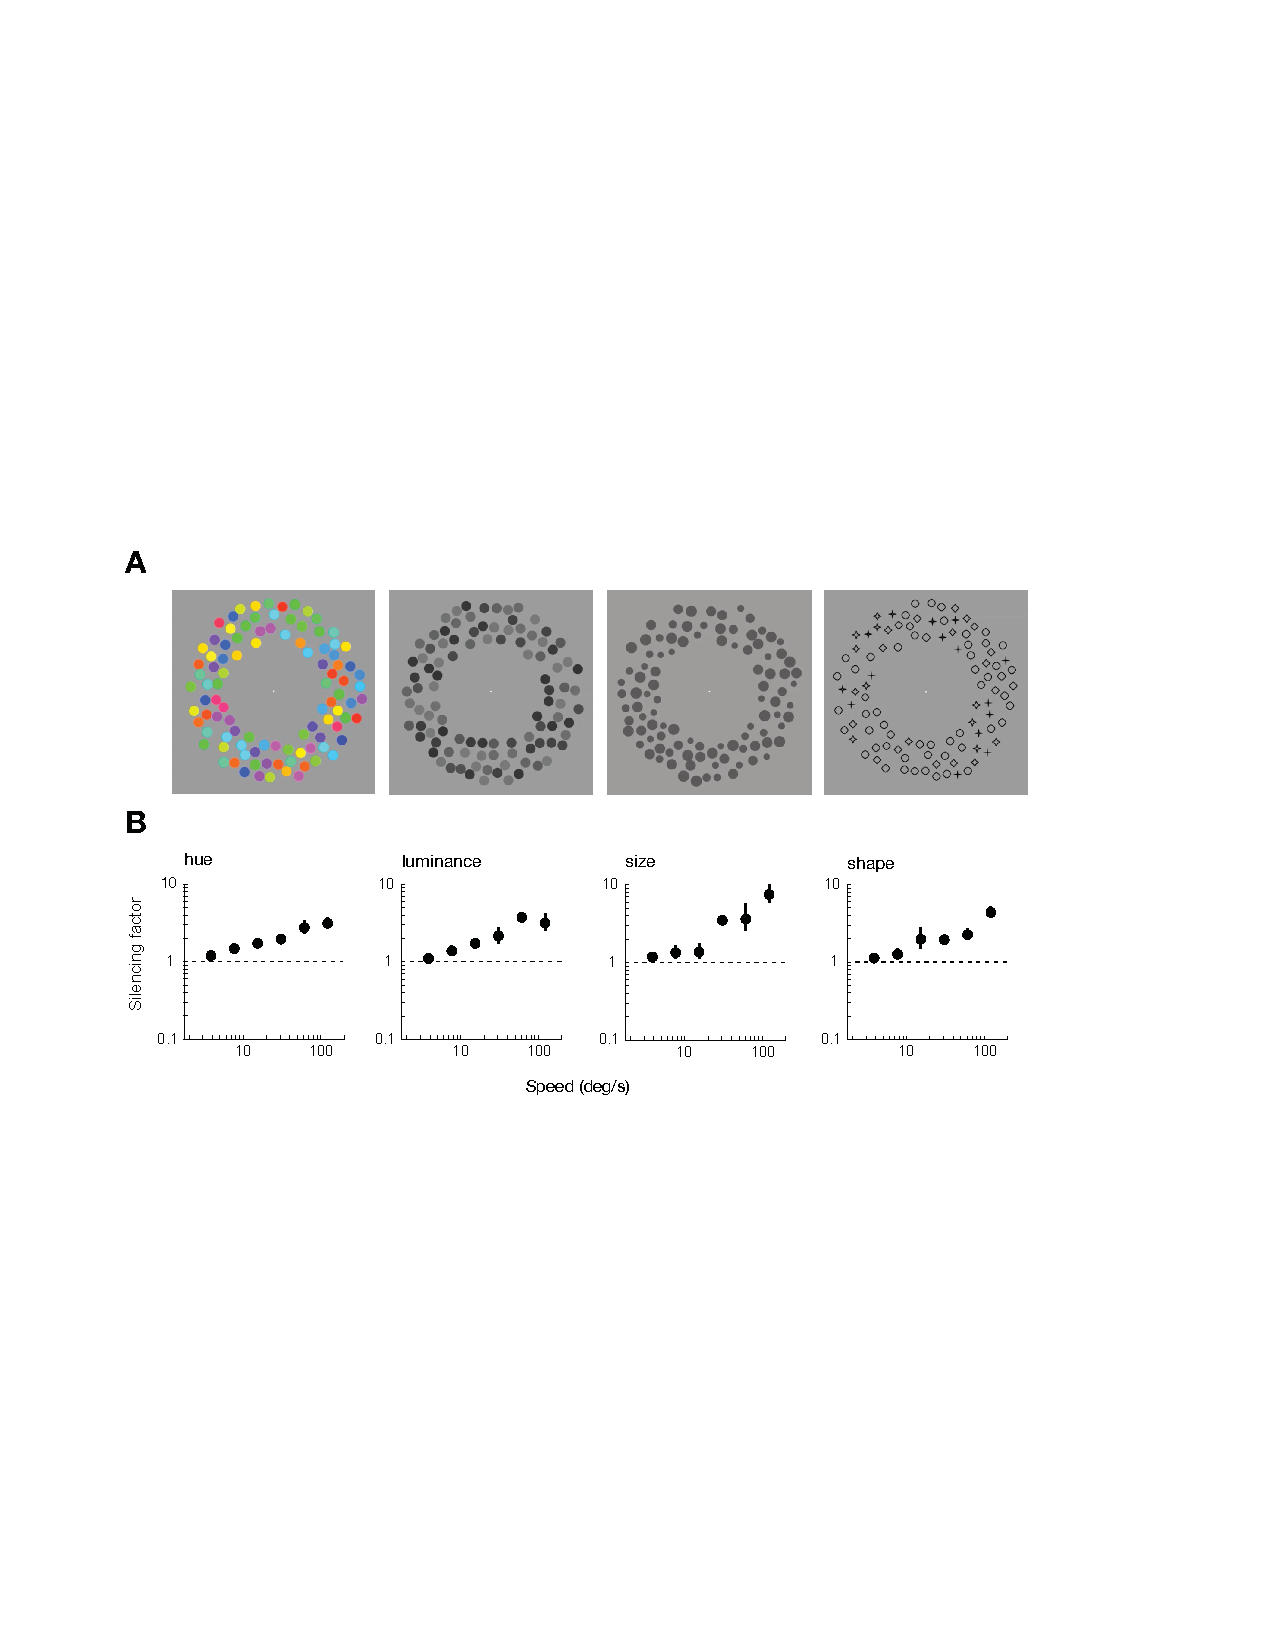
\includegraphics[width=\textwidth]{figures/fig1}
\caption[Short figure name.]{This is a figure that floats inline and here is its caption.
\label{fig:myInlineFigure}}
\end{figure}


Quisque facilisis erat a dui. Nam malesuada ornare dolor. Cras gravida, diam sit amet rhoncus ornare, erat elit consectetuer erat, id egestas pede nibh eget odio. Proin tincidunt, velit vel porta elementum, magna diam molestie sapien, non aliquet massa pede eu diam. Aliquam iaculis. Fusce et ipsum et nulla tristique facilisis. Donec eget sem sit amet ligula viverra gravida. Etiam vehicula urna vel turpis. Suspendisse sagittis ante a urna. Morbi a est quis orci consequat rutrum. Nullam egestas feugiat felis. Integer adipiscing semper ligula. Nunc molestie, nisl sit amet cursus convallis, sapien lectus pretium metus, vitae pretium enim wisi id lectus. Donec vestibulum. Etiam vel nibh. Nulla facilisi. Mauris pharetra. Donec augue. Fusce ultrices, neque id dignissim ultrices, tellus mauris dictum elit, vel lacinia enim metus eu nunc.

Proin at eros non eros adipiscing mollis. Donec semper turpis sed diam. Sed consequat ligula nec tortor. Integer eget sem. Ut vitae enim eu est vehicula gravida. Morbi ipsum ipsum, porta nec, tempor id, auctor vitae, purus. Pellentesque neque. Nulla luctus erat vitae libero. Integer nec enim. Phasellus aliquam enim et tortor. Quisque aliquet, quam elementum condimentum feugiat, tellus odio consectetuer wisi, vel nonummy sem neque in elit. Curabitur eleifend wisi iaculis ipsum. Pellentesque habitant morbi tristique senectus et netus et malesuada fames ac turpis egestas. In non velit non ligula laoreet ultrices. Praesent ultricies facilisis nisl. Vivamus luctus elit sit amet mi. Phasellus pellentesque, erat eget elementum volutpat, dolor nisl porta neque, vitae sodales ipsum nibh in ligula. Maecenas mattis pulvinar diam. Curabitur sed leo.

Nulla facilisi. In vel sem. Morbi id urna in diam dignissim feugiat. Proin molestie tortor eu velit. Aliquam erat volutpat. Nullam ultrices, diam tempus vulputate egestas, eros pede varius leo, sed imperdiet lectus est ornare odio. Lorem ipsum dolor sit amet, consectetuer adipiscing elit. Proin consectetuer velit in dui. Phasellus wisi purus, interdum vitae, rutrum accumsan, viverra in, velit. Sed enim risus, congue non, tristique in, commodo eu, metus. Aenean tortor mi, imperdiet id, gravida eu, posuere eu, felis. Mauris sollicitudin, turpis in hendrerit sodales, lectus ipsum pellentesque ligula, sit amet scelerisque urna nibh ut arcu. Aliquam in lacus. Vestibulum ante ipsum primis in faucibus orci luctus et ultrices posuere cubilia Curae; Nulla placerat aliquam wisi. Mauris viverra odio. Quisque fermentum pulvinar odio. Proin posuere est vitae ligula. Etiam euismod. Cras a eros.

Nunc auctor bibendum eros. Maecenas porta accumsan mauris. Etiam enim enim, elementum sed, bibendum quis, rhoncus non, metus. Fusce neque dolor, adipiscing sed, consectetuer et, lacinia sit amet, quam. Suspendisse wisi quam, consectetuer in, blandit sed, suscipit eu, eros. Etiam ligula enim, tempor ut, blandit nec, mollis eu, lectus. Nam cursus. Vivamus iaculis. Aenean risus purus, pharetra in, blandit quis, gravida a, turpis. Donec nisl. Aenean eget mi. Fusce mattis est id diam. Phasellus faucibus interdum sapien. Duis quis nunc. Sed enim.

Pellentesque vel dui sed orci faucibus iaculis. Suspendisse dictum magna id purus tincidunt rutrum. Nulla congue. Vivamus sit amet lorem posuere dui vulputate ornare. Phasellus mattis sollicitudin ligula. Duis dignissim felis et urna. Integer adipiscing congue metus. Nam pede. Etiam non wisi. Sed accumsan dolor ac augue. Pellentesque eget lectus. Aliquam nec dolor nec tellus ornare venenatis. Nullam blandit placerat sem. Curabitur quis ipsum. Mauris nisl tellus, aliquet eu, suscipit eu, ullamcorper quis, magna. Mauris elementum, pede at sodales vestibulum, nulla tortor congue massa, quis pellentesque odio dui id est. Cras faucibus augue.

%% Requires fltpage2 package
%%
% \begin{FPfigure}
% 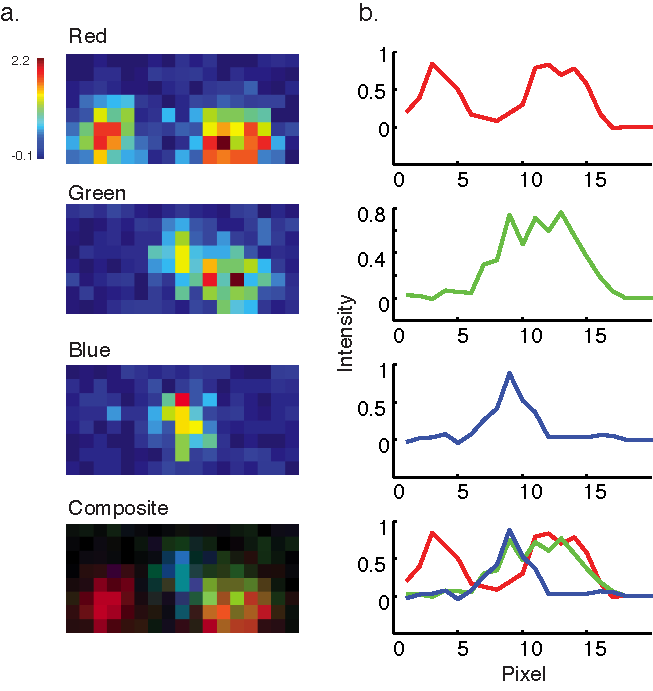
\includegraphics[width=\textwidth]{figures/fullpage}
% \caption[Short figure name.]{This is a full page figure using the FPfigure command. It takes up the whole page and the caption appears on the preceding page. Its useful for large figures. Harvard's rules about full page figures are tricky, but you don't have to worry about it because we took care of it for you. For example, the full figure is supposed to have a title in the same style as the caption but without the actual caption. The caption is supposed to appear alone on the preceding page with no other text. You do't have to worry about any of that. We have modified the fltpage package to make it work. This is a lengthy caption and it clearly would not fit on the same page as the figure. Note that you should only use the FPfigure command in instances where the figure really is too large. If the figure is small enough to fit by the caption than it does not produce the desired effect. Good luck with your thesis. I have to keep writing this to make the caption really long. LaTex is a lot of fun. You will enjoy working with it. Good luck on your post doctoral life! I am looking forward to mine. \label{fig:myFullPageFigure}}
% \end{FPfigure}
% \afterpage{\clearpage}

Suspendisse vestibulum dignissim quam. Integer vel augue. Phasellus nulla purus, interdum ac, venenatis non, varius rutrum, leo. Pellentesque habitant morbi tristique senectus et netus et malesuada fames ac turpis egestas. Duis a eros. Class aptent taciti sociosqu ad litora torquent per conubia nostra, per inceptos hymenaeos. Fusce magna mi, porttitor quis, convallis eget, sodales ac, urna. Phasellus luctus venenatis magna. Vivamus eget lacus. Nunc tincidunt convallis tortor. Duis eros mi, dictum vel, fringilla sit amet, fermentum id, sem. Phasellus nunc enim, faucibus ut, laoreet in, consequat id, metus. Vivamus dignissim. Cras lobortis tempor velit. Phasellus nec diam ac nisl lacinia tristique. Nullam nec metus id mi dictum dignissim. Nullam quis wisi non sem lobortis condimentum. Phasellus pulvinar, nulla non aliquam eleifend, tortor wisi scelerisque felis, in sollicitudin arcu ante lacinia leo.

Pellentesque habitant morbi tristique senectus et netus et malesuada fames ac turpis egestas. Vestibulum tortor quam, feugiat vitae, ultricies eget, tempor sit amet, ante. Donec eu libero sit amet quam egestas semper. Aenean ultricies mi vitae est. Mauris placerat eleifend leo. Quisque sit amet est et sapien ullamcorper pharetra. Vestibulum erat wisi, condimentum sed, commodo vitae, ornare sit amet, wisi. Aenean fermentum, elit eget tincidunt condimentum, eros ipsum rutrum orci, sagittis tempus lacus enim ac dui. Donec non enim in turpis pulvinar facilisis. Ut felis.

Cras sed ante. Phasellus in massa. Curabitur dolor eros, gravida et, hendrerit ac, cursus non, massa. Aliquam lorem. In hac habitasse platea dictumst. Cras eu mauris. Quisque lacus. Donec ipsum. Nullam vitae sem at nunc pharetra ultricies. Vivamus elit eros, ullamcorper a, adipiscing sit amet, porttitor ut, nibh. Maecenas adipiscing mollis massa. Nunc ut dui eget nulla venenatis aliquet. Sed luctus posuere justo. Cras vehicula varius turpis. Vivamus eros metus, tristique sit amet, molestie dignissim, malesuada et, urna.

Proin at eros non eros adipiscing mollis. Donec semper turpis sed diam. Sed consequat ligula nec tortor. Integer eget sem. Ut vitae enim eu est vehicula gravida. Morbi ipsum ipsum, porta nec, tempor id, auctor vitae, purus. Pellentesque neque. Nulla luctus erat vitae libero. Integer nec enim. Phasellus aliquam enim et tortor. Quisque aliquet, quam elementum condimentum feugiat, tellus odio consectetuer wisi, vel nonummy sem neque in elit. Curabitur eleifend wisi iaculis ipsum. Pellentesque habitant morbi tristique senectus et netus et malesuada fames ac turpis egestas. In non velit non ligula laoreet ultrices. Praesent ultricies facilisis nisl. Vivamus luctus elit sit amet mi. Phasellus pellentesque, erat eget elementum volutpat, dolor nisl porta neque, vitae sodales ipsum nibh in ligula. Maecenas mattis pulvinar diam. Curabitur sed leo.

Nulla facilisi. In vel sem. Morbi id urna in diam dignissim feugiat. Proin molestie tortor eu velit. Aliquam erat volutpat. Nullam ultrices, diam tempus vulputate egestas, eros pede varius leo, sed imperdiet lectus est ornare odio. Lorem ipsum dolor sit amet, consectetuer adipiscing elit. Proin consectetuer velit in dui. Phasellus wisi purus, interdum vitae, rutrum accumsan, viverra in, velit. Sed enim risus, congue non, tristique in, commodo eu, metus. Aenean tortor mi, imperdiet id, gravida eu, posuere eu, felis. Mauris sollicitudin, turpis in hendrerit sodales, lectus ipsum pellentesque ligula, sit amet scelerisque urna nibh ut arcu. Aliquam in lacus. Vestibulum ante ipsum primis in faucibus orci luctus et ultrices posuere cubilia Curae; Nulla placerat aliquam wisi. Mauris viverra odio. Quisque fermentum pulvinar odio. Proin posuere est vitae ligula. Etiam euismod. Cras a eros.

Nunc auctor bibendum eros. Maecenas porta accumsan mauris. Etiam enim enim, elementum sed, bibendum quis, rhoncus non, metus. Fusce neque dolor, adipiscing sed, consectetuer et, lacinia sit amet, quam. Suspendisse wisi quam, consectetuer in, blandit sed, suscipit eu, eros. Etiam ligula enim, tempor ut, blandit nec, mollis eu, lectus. Nam cursus. Vivamus iaculis. Aenean risus purus, pharetra in, blandit quis, gravida a, turpis. Donec nisl. Aenean eget mi. Fusce mattis est id diam. Phasellus faucibus interdum sapien. Duis quis nunc. Sed enim.

Pellentesque vel dui sed orci faucibus iaculis. Suspendisse dictum magna id purus tincidunt rutrum. Nulla congue. Vivamus sit amet lorem posuere dui vulputate ornare. Phasellus mattis sollicitudin ligula. Duis dignissim felis et urna. Integer adipiscing congue metus. Nam pede. Etiam non wisi. Sed accumsan dolor ac augue. Pellentesque eget lectus. Aliquam nec dolor nec tellus ornare venenatis. Nullam blandit placerat sem. Curabitur quis ipsum. Mauris nisl tellus, aliquet eu, suscipit eu, ullamcorper quis, magna. Mauris elementum, pede at sodales vestibulum, nulla tortor congue massa, quis pellentesque odio dui id est. Cras faucibus augue.

Suspendisse vestibulum dignissim quam. Integer vel augue. Phasellus nulla purus, interdum ac, venenatis non, varius rutrum, leo. Pellentesque habitant morbi tristique senectus et netus et malesuada fames ac turpis egestas. Duis a eros. Class aptent taciti sociosqu ad litora torquent per conubia nostra, per inceptos hymenaeos. Fusce magna mi, porttitor quis, convallis eget, sodales ac, urna. Phasellus luctus venenatis magna. Vivamus eget lacus. Nunc tincidunt convallis tortor. Duis eros mi, dictum vel, fringilla sit amet, fermentum id, sem. Phasellus nunc enim, faucibus ut, laoreet in, consequat id, metus. Vivamus dignissim. Cras lobortis tempor velit. Phasellus nec diam ac nisl lacinia tristique. Nullam nec metus id mi dictum dignissim. Nullam quis wisi non sem lobortis condimentum. Phasellus pulvinar, nulla non aliquam eleifend, tortor wisi scelerisque felis, in sollicitudin arcu ante lacinia leo.

Pellentesque habitant morbi tristique senectus et netus et malesuada fames ac turpis egestas. Vestibulum tortor quam, feugiat vitae, ultricies eget, tempor sit amet, ante. Donec eu libero sit amet quam egestas semper. Aenean ultricies mi vitae est. Mauris placerat eleifend leo. Quisque sit amet est et sapien ullamcorper pharetra. Vestibulum erat wisi, condimentum sed, commodo vitae, ornare sit amet, wisi. Aenean fermentum, elit eget tincidunt condimentum, eros ipsum rutrum orci, sagittis tempus lacus enim ac dui. Donec non enim in turpis pulvinar facilisis. Ut felis.

Cras sed ante. Phasellus in massa. Curabitur dolor eros, gravida et, hendrerit ac, cursus non, massa. Aliquam lorem. In hac habitasse platea dictumst. Cras eu mauris. Quisque lacus. Donec ipsum. Nullam vitae sem at nunc pharetra ultricies. Vivamus elit eros, ullamcorper a, adipiscing sit amet, porttitor ut, nibh. Maecenas adipiscing mollis massa. Nunc ut dui eget nulla venenatis aliquet. Sed luctus posuere justo. Cras vehicula varius turpis. Vivamus eros metus, tristique sit amet, molestie dignissim, malesuada et, urna.

Cras dictum. Maecenas ut turpis. In vitae erat ac orci dignissim eleifend. Nunc quis justo. Sed vel ipsum in purus tincidunt pharetra. Sed pulvinar, felis id consectetuer malesuada, enim nisl mattis elit, a facilisis tortor nibh quis leo. Sed augue lacus, pretium vitae, molestie eget, rhoncus quis, elit. Donec in augue. Fusce orci wisi, ornare id, mollis vel, lacinia vel, massa.

Lorem ipsum dolor sit amet, consectetuer adipiscing elit. Morbi commodo, ipsum sed pharetra gravida, orci magna rhoncus neque, id pulvinar odio lorem non turpis. Nullam sit amet enim. Suspendisse id velit vitae ligula volutpat condimentum. Aliquam erat volutpat. Sed quis velit. Nulla facilisi. Nulla libero. Vivamus pharetra posuere sapien. Nam consectetuer. Sed aliquam, nunc eget euismod ullamcorper, lectus nunc ullamcorper orci, fermentum bibendum enim nibh eget ipsum. Donec porttitor ligula eu dolor. Maecenas vitae nulla consequat libero cursus venenatis. Nam magna enim, accumsan eu, blandit sed, blandit a, eros.

Quisque facilisis erat a dui. Nam malesuada ornare dolor. Cras gravida, diam sit amet rhoncus ornare, erat elit consectetuer erat, id egestas pede nibh eget odio. Proin tincidunt, velit vel porta elementum, magna diam molestie sapien, non aliquet massa pede eu diam. Aliquam iaculis. Fusce et ipsum et nulla tristique facilisis. Donec eget sem sit amet ligula viverra gravida. Etiam vehicula urna vel turpis. Suspendisse sagittis ante a urna. Morbi a est quis orci consequat rutrum. Nullam egestas feugiat felis. Integer adipiscing semper ligula. Nunc molestie, nisl sit amet cursus convallis, sapien lectus pretium metus, vitae pretium enim wisi id lectus. Donec vestibulum. Etiam vel nibh. Nulla facilisi. Mauris pharetra. Donec augue. Fusce ultrices, neque id dignissim ultrices, tellus mauris dictum elit, vel lacinia enim metus eu nunc.

Proin at eros non eros adipiscing mollis. Donec semper turpis sed diam. Sed consequat ligula nec tortor. Integer eget sem. Ut vitae enim eu est vehicula gravida. Morbi ipsum ipsum, porta nec, tempor id, auctor vitae, purus. Pellentesque neque. Nulla luctus erat vitae libero. Integer nec enim. Phasellus aliquam enim et tortor. Quisque aliquet, quam elementum condimentum feugiat, tellus odio consectetuer wisi, vel nonummy sem neque in elit. Curabitur eleifend wisi iaculis ipsum. Pellentesque habitant morbi tristique senectus et netus et malesuada fames ac turpis egestas. In non velit non ligula laoreet ultrices. Praesent ultricies facilisis nisl. Vivamus luctus elit sit amet mi. Phasellus pellentesque, erat eget elementum volutpat, dolor nisl porta neque, vitae sodales ipsum nibh in ligula. Maecenas mattis pulvinar diam. Curabitur sed leo.

Nulla facilisi. In vel sem. Morbi id urna in diam dignissim feugiat. Proin molestie tortor eu velit. Aliquam erat volutpat. Nullam ultrices, diam tempus vulputate egestas, eros pede varius leo, sed imperdiet lectus est ornare odio. Lorem ipsum dolor sit amet, consectetuer adipiscing elit. Proin consectetuer velit in dui. Phasellus wisi purus, interdum vitae, rutrum accumsan, viverra in, velit. Sed enim risus, congue non, tristique in, commodo eu, metus. Aenean tortor mi, imperdiet id, gravida eu, posuere eu, felis. Mauris sollicitudin, turpis in hendrerit sodales, lectus ipsum pellentesque ligula, sit amet scelerisque urna nibh ut arcu. Aliquam in lacus. Vestibulum ante ipsum primis in faucibus orci luctus et ultrices posuere cubilia Curae; Nulla placerat aliquam wisi. Mauris viverra odio. Quisque fermentum pulvinar odio. Proin posuere est vitae ligula. Etiam euismod. Cras a eros.

Nunc auctor bibendum eros. Maecenas porta accumsan mauris. Etiam enim enim, elementum sed, bibendum quis, rhoncus non, metus. Fusce neque dolor, adipiscing sed, consectetuer et, lacinia sit amet, quam. Suspendisse wisi quam, consectetuer in, blandit sed, suscipit eu, eros. Etiam ligula enim, tempor ut, blandit nec, mollis eu, lectus. Nam cursus. Vivamus iaculis. Aenean risus purus, pharetra in, blandit quis, gravida a, turpis. Donec nisl. Aenean eget mi. Fusce mattis est id diam. Phasellus faucibus interdum sapien. Duis quis nunc. Sed enim.

Pellentesque vel dui sed orci faucibus iaculis. Suspendisse dictum magna id purus tincidunt rutrum. Nulla congue. Vivamus sit amet lorem posuere dui vulputate ornare. Phasellus mattis sollicitudin ligula. Duis dignissim felis et urna. Integer adipiscing congue metus. Nam pede. Etiam non wisi. Sed accumsan dolor ac augue. Pellentesque eget lectus. Aliquam nec dolor nec tellus ornare venenatis. Nullam blandit placerat sem. Curabitur quis ipsum. Mauris nisl tellus, aliquet eu, suscipit eu, ullamcorper quis, magna. Mauris elementum, pede at sodales vestibulum, nulla tortor congue massa, quis pellentesque odio dui id est. Cras faucibus augue.

Suspendisse vestibulum dignissim quam. Integer vel augue. Phasellus nulla purus, interdum ac, venenatis non, varius rutrum, leo. Pellentesque habitant morbi tristique senectus et netus et malesuada fames ac turpis egestas. Duis a eros. Class aptent taciti sociosqu ad litora torquent per conubia nostra, per inceptos hymenaeos. Fusce magna mi, porttitor quis, convallis eget, sodales ac, urna. Phasellus luctus venenatis magna. Vivamus eget lacus. Nunc tincidunt convallis tortor. Duis eros mi, dictum vel, fringilla sit amet, fermentum id, sem. Phasellus nunc enim, faucibus ut, laoreet in, consequat id, metus. Vivamus dignissim. Cras lobortis tempor velit. Phasellus nec diam ac nisl lacinia tristique. Nullam nec metus id mi dictum dignissim. Nullam quis wisi non sem lobortis condimentum. Phasellus pulvinar, nulla non aliquam eleifend, tortor wisi scelerisque felis, in sollicitudin arcu ante lacinia leo.

Pellentesque habitant morbi tristique senectus et netus et malesuada fames ac turpis egestas. Vestibulum tortor quam, feugiat vitae, ultricies eget, tempor sit amet, ante. Donec eu libero sit amet quam egestas semper. Aenean ultricies mi vitae est. Mauris placerat eleifend leo. Quisque sit amet est et sapien ullamcorper pharetra. Vestibulum erat wisi, condimentum sed, commodo vitae, ornare sit amet, wisi. Aenean fermentum, elit eget tincidunt condimentum, eros ipsum rutrum orci, sagittis tempus lacus enim ac dui. Donec non enim in turpis pulvinar facilisis. Ut felis.

Cras sed ante. Phasellus in massa. Curabitur dolor eros, gravida et, hendrerit ac, cursus non, massa. Aliquam lorem. In hac habitasse platea dictumst. Cras eu mauris. Quisque lacus. Donec ipsum. Nullam vitae sem at nunc pharetra ultricies. Vivamus elit eros, ullamcorper a, adipiscing sit amet, porttitor ut, nibh. Maecenas adipiscing mollis massa. Nunc ut dui eget nulla venenatis aliquet. Sed luctus posuere justo. Cras vehicula varius turpis. Vivamus eros metus, tristique sit amet, molestie dignissim, malesuada et, urna.

Cras dictum. Maecenas ut turpis. In vitae erat ac orci dignissim eleifend. Nunc quis justo. Sed vel ipsum in purus tincidunt pharetra. Sed pulvinar, felis id consectetuer malesuada, enim nisl mattis elit, a facilisis tortor nibh quis leo. Sed augue lacus, pretium vitae, molestie eget, rhoncus quis, elit. Donec in augue. Fusce orci wisi, ornare id, mollis vel, lacinia vel, massa.

Lorem ipsum dolor sit amet, consectetuer adipiscing elit. Morbi commodo, ipsum sed pharetra gravida, orci magna rhoncus neque, id pulvinar odio lorem non turpis. Nullam sit amet enim. Suspendisse id velit vitae ligula volutpat condimentum. Aliquam erat volutpat. Sed quis velit. Nulla facilisi. Nulla libero. Vivamus pharetra posuere sapien. Nam consectetuer. Sed aliquam, nunc eget euismod ullamcorper, lectus nunc ullamcorper orci, fermentum bibendum enim nibh eget ipsum. Donec porttitor ligula eu dolor. Maecenas vitae nulla consequat libero cursus venenatis. Nam magna enim, accumsan eu, blandit sed, blandit a, eros.

Quisque facilisis erat a dui. Nam malesuada ornare dolor. Cras gravida, diam sit amet rhoncus ornare, erat elit consectetuer erat, id egestas pede nibh eget odio. Proin tincidunt, velit vel porta elementum, magna diam molestie sapien, non aliquet massa pede eu diam. Aliquam iaculis. Fusce et ipsum et nulla tristique facilisis. Donec eget sem sit amet ligula viverra gravida. Etiam vehicula urna vel turpis. Suspendisse sagittis ante a urna. Morbi a est quis orci consequat rutrum. Nullam egestas feugiat felis. Integer adipiscing semper ligula. Nunc molestie, nisl sit amet cursus convallis, sapien lectus pretium metus, vitae pretium enim wisi id lectus. Donec vestibulum. Etiam vel nibh. Nulla facilisi. Mauris pharetra. Donec augue. Fusce ultrices, neque id dignissim ultrices, tellus mauris dictum elit, vel lacinia enim metus eu nunc.

Proin at eros non eros adipiscing mollis. Donec semper turpis sed diam. Sed consequat ligula nec tortor. Integer eget sem. Ut vitae enim eu est vehicula gravida. Morbi ipsum ipsum, porta nec, tempor id, auctor vitae, purus. Pellentesque neque. Nulla luctus erat vitae libero. Integer nec enim. Phasellus aliquam enim et tortor. Quisque aliquet, quam elementum condimentum feugiat, tellus odio consectetuer wisi, vel nonummy sem neque in elit. Curabitur eleifend wisi iaculis ipsum. Pellentesque habitant morbi tristique senectus et netus et malesuada fames ac turpis egestas. In non velit non ligula laoreet ultrices. Praesent ultricies facilisis nisl. Vivamus luctus elit sit amet mi. Phasellus pellentesque, erat eget elementum volutpat, dolor nisl porta neque, vitae sodales ipsum nibh in ligula. Maecenas mattis pulvinar diam. Curabitur sed leo.

Nulla facilisi. In vel sem. Morbi id urna in diam dignissim feugiat. Proin molestie tortor eu velit. Aliquam erat volutpat. Nullam ultrices, diam tempus vulputate egestas, eros pede varius leo, sed imperdiet lectus est ornare odio. Lorem ipsum dolor sit amet, consectetuer adipiscing elit. Proin consectetuer velit in dui. Phasellus wisi purus, interdum vitae, rutrum accumsan, viverra in, velit. Sed enim risus, congue non, tristique in, commodo eu, metus. Aenean tortor mi, imperdiet id, gravida eu, posuere eu, felis. Mauris sollicitudin, turpis in hendrerit sodales, lectus ipsum pellentesque ligula, sit amet scelerisque urna nibh ut arcu. Aliquam in lacus. Vestibulum ante ipsum primis in faucibus orci luctus et ultrices posuere cubilia Curae; Nulla placerat aliquam wisi. Mauris viverra odio. Quisque fermentum pulvinar odio. Proin posuere est vitae ligula. Etiam euismod. Cras a eros.

Nunc auctor bibendum eros. Maecenas porta accumsan mauris. Etiam enim enim, elementum sed, bibendum quis, rhoncus non, metus. Fusce neque dolor, adipiscing sed, consectetuer et, lacinia sit amet, quam. Suspendisse wisi quam, consectetuer in, blandit sed, suscipit eu, eros. Etiam ligula enim, tempor ut, blandit nec, mollis eu, lectus. Nam cursus. Vivamus iaculis. Aenean risus purus, pharetra in, blandit quis, gravida a, turpis. Donec nisl. Aenean eget mi. Fusce mattis est id diam. Phasellus faucibus interdum sapien. Duis quis nunc. Sed enim.


Cras sed ante. Phasellus in massa. Curabitur dolor eros, gravida et, hendrerit ac, cursus non, massa. Aliquam lorem. In hac habitasse platea dictumst. Cras eu mauris. Quisque lacus. Donec ipsum. Nullam vitae sem at nunc pharetra ultricies. Vivamus elit eros, ullamcorper a, adipiscing sit amet, porttitor ut, nibh. Maecenas adipiscing mollis massa. Nunc ut dui eget nulla venenatis aliquet. Sed luctus posuere justo. Cras vehicula varius turpis. Vivamus eros metus, tristique sit amet, molestie dignissim, malesuada et, urna.

Cras dictum. Maecenas ut turpis. In vitae erat ac orci dignissim eleifend. Nunc quis justo. Sed vel ipsum in purus tincidunt pharetra. Sed pulvinar, felis id consectetuer malesuada, enim nisl mattis elit, a facilisis tortor nibh quis leo. Sed augue lacus, pretium vitae, molestie eget, rhoncus quis, elit. Donec in augue. Fusce orci wisi, ornare id, mollis vel, lacinia vel, massa.

Lorem ipsum dolor sit amet, consectetuer adipiscing elit. Morbi commodo, ipsum sed pharetra gravida, orci magna rhoncus neque, id pulvinar odio lorem non turpis. Nullam sit amet enim. Suspendisse id velit vitae ligula volutpat condimentum. Aliquam erat volutpat. Sed quis velit. Nulla facilisi. Nulla libero. Vivamus pharetra posuere sapien. Nam consectetuer. Sed aliquam, nunc eget euismod ullamcorper, lectus nunc ullamcorper orci, fermentum bibendum enim nibh eget ipsum. Donec porttitor ligula eu dolor. Maecenas vitae nulla consequat libero cursus venenatis. Nam magna enim, accumsan eu, blandit sed, blandit a, eros.

Quisque facilisis erat a dui. Nam malesuada ornare dolor. Cras gravida, diam sit amet rhoncus ornare, erat elit consectetuer erat, id egestas pede nibh eget odio. Proin tincidunt, velit vel porta elementum, magna diam molestie sapien, non aliquet massa pede eu diam. Aliquam iaculis. Fusce et ipsum et nulla tristique facilisis. Donec eget sem sit amet ligula viverra gravida. Etiam vehicula urna vel turpis. Suspendisse sagittis ante a urna. Morbi a est quis orci consequat rutrum. Nullam egestas feugiat felis. Integer adipiscing semper ligula. Nunc molestie, nisl sit amet cursus convallis, sapien lectus pretium metus, vitae pretium enim wisi id lectus. Donec vestibulum. Etiam vel nibh. Nulla facilisi. Mauris pharetra. Donec augue. Fusce ultrices, neque id dignissim ultrices, tellus mauris dictum elit, vel lacinia enim metus eu nunc.

Proin at eros non eros adipiscing mollis. Donec semper turpis sed diam. Sed consequat ligula nec tortor. Integer eget sem. Ut vitae enim eu est vehicula gravida. Morbi ipsum ipsum, porta nec, tempor id, auctor vitae, purus. Pellentesque neque. Nulla luctus erat vitae libero. Integer nec enim. Phasellus aliquam enim et tortor. Quisque aliquet, quam elementum condimentum feugiat, tellus odio consectetuer wisi, vel nonummy sem neque in elit. Curabitur eleifend wisi iaculis ipsum. Pellentesque habitant morbi tristique senectus et netus et malesuada fames ac turpis egestas. In non velit non ligula laoreet ultrices. Praesent ultricies facilisis nisl. Vivamus luctus elit sit amet mi. Phasellus pellentesque, erat eget elementum volutpat, dolor nisl porta neque, vitae sodales ipsum nibh in ligula. Maecenas mattis pulvinar diam. Curabitur sed leo.

Nulla facilisi. In vel sem. Morbi id urna in diam dignissim feugiat. Proin molestie tortor eu velit. Aliquam erat volutpat. Nullam ultrices, diam tempus vulputate egestas, eros pede varius leo, sed imperdiet lectus est ornare odio. Lorem ipsum dolor sit amet, consectetuer adipiscing elit. Proin consectetuer velit in dui. Phasellus wisi purus, interdum vitae, rutrum accumsan, viverra in, velit. Sed enim risus, congue non, tristique in, commodo eu, metus. Aenean tortor mi, imperdiet id, gravida eu, posuere eu, felis. Mauris sollicitudin, turpis in hendrerit sodales, lectus ipsum pellentesque ligula, sit amet scelerisque urna nibh ut arcu. Aliquam in lacus. Vestibulum ante ipsum primis in faucibus orci luctus et ultrices posuere cubilia Curae; Nulla placerat aliquam wisi. Mauris viverra odio. Quisque fermentum pulvinar odio. Proin posuere est vitae ligula. Etiam euismod. Cras a eros.

Nunc auctor bibendum eros. Maecenas porta accumsan mauris. Etiam enim enim, elementum sed, bibendum quis, rhoncus non, metus. Fusce neque dolor, adipiscing sed, consectetuer et, lacinia sit amet, quam. Suspendisse wisi quam, consectetuer in, blandit sed, suscipit eu, eros. Etiam ligula enim, tempor ut, blandit nec, mollis eu, lectus. Nam cursus. Vivamus iaculis. Aenean risus purus, pharetra in, blandit quis, gravida a, turpis. Donec nisl. Aenean eget mi. Fusce mattis est id diam. Phasellus faucibus interdum sapien. Duis quis nunc. Sed enim.

Pellentesque vel dui sed orci faucibus iaculis. Suspendisse dictum magna id purus tincidunt rutrum. Nulla congue. Vivamus sit amet lorem posuere dui vulputate ornare. Phasellus mattis sollicitudin ligula. Duis dignissim felis et urna. Integer adipiscing congue metus. Nam pede. Etiam non wisi. Sed accumsan dolor ac augue. Pellentesque eget lectus. Aliquam nec dolor nec tellus ornare venenatis. Nullam blandit placerat sem. Curabitur quis ipsum. Mauris nisl tellus, aliquet eu, suscipit eu, ullamcorper quis, magna. Mauris elementum, pede at sodales vestibulum, nulla tortor congue massa, quis pellentesque odio dui id est. Cras faucibus augue.

Suspendisse vestibulum dignissim quam. Integer vel augue. Phasellus nulla purus, interdum ac, venenatis non, varius rutrum, leo. Pellentesque habitant morbi tristique senectus et netus et malesuada fames ac turpis egestas. Duis a eros. Class aptent taciti sociosqu ad litora torquent per conubia nostra, per inceptos hymenaeos. Fusce magna mi, porttitor quis, convallis eget, sodales ac, urna. Phasellus luctus venenatis magna. Vivamus eget lacus. Nunc tincidunt convallis tortor. Duis eros mi, dictum vel, fringilla sit amet, fermentum id, sem. Phasellus nunc enim, faucibus ut, laoreet in, consequat id, metus. Vivamus dignissim. Cras lobortis tempor velit. Phasellus nec diam ac nisl lacinia tristique. Nullam nec metus id mi dictum dignissim. Nullam quis wisi non sem lobortis condimentum. Phasellus pulvinar, nulla non aliquam eleifend, tortor wisi scelerisque felis, in sollicitudin arcu ante lacinia leo.

Pellentesque habitant morbi tristique senectus et netus et malesuada fames ac turpis egestas. Vestibulum tortor quam, feugiat vitae, ultricies eget, tempor sit amet, ante. Donec eu libero sit amet quam egestas semper. Aenean ultricies mi vitae est. Mauris placerat eleifend leo. Quisque sit amet est et sapien ullamcorper pharetra. Vestibulum erat wisi, condimentum sed, commodo vitae, ornare sit amet, wisi. Aenean fermentum, elit eget tincidunt condimentum, eros ipsum rutrum orci, sagittis tempus lacus enim ac dui. Donec non enim in turpis pulvinar facilisis. Ut felis.

Cras sed ante. Phasellus in massa. Curabitur dolor eros, gravida et, hendrerit ac, cursus non, massa. Aliquam lorem. In hac habitasse platea dictumst. Cras eu mauris. Quisque lacus. Donec ipsum. Nullam vitae sem at nunc pharetra ultricies. Vivamus elit eros, ullamcorper a, adipiscing sit amet, porttitor ut, nibh. Maecenas adipiscing mollis massa. Nunc ut dui eget nulla venenatis aliquet. Sed luctus posuere justo. Cras vehicula varius turpis. Vivamus eros metus, tristique sit amet, molestie dignissim, malesuada et, urna.

Cras dictum. Maecenas ut turpis. In vitae erat ac orci dignissim eleifend. Nunc quis justo. Sed vel ipsum in purus tincidunt pharetra. Sed pulvinar, felis id consectetuer malesuada, enim nisl mattis elit, a facilisis tortor nibh quis leo. Sed augue lacus, pretium vitae, molestie eget, rhoncus quis, elit. Donec in augue. Fusce orci wisi, ornare id, mollis vel, lacinia vel, massa.

Lorem ipsum dolor sit amet, consectetuer adipiscing elit. Morbi commodo, ipsum sed pharetra gravida, orci magna rhoncus neque, id pulvinar odio lorem non turpis. Nullam sit amet enim. Suspendisse id velit vitae ligula volutpat condimentum. Aliquam erat volutpat. Sed quis velit. Nulla facilisi. Nulla libero. Vivamus pharetra posuere sapien. Nam consectetuer. Sed aliquam, nunc eget euismod ullamcorper, lectus nunc ullamcorper orci, fermentum bibendum enim nibh eget ipsum. Donec porttitor ligula eu dolor. Maecenas vitae nulla consequat libero cursus venenatis. Nam magna enim, accumsan eu, blandit sed, blandit a, eros.

Quisque facilisis erat a dui. Nam malesuada ornare dolor. Cras gravida, diam sit amet rhoncus ornare, erat elit consectetuer erat, id egestas pede nibh eget odio. Proin tincidunt, velit vel porta elementum, magna diam molestie sapien, non aliquet massa pede eu diam. Aliquam iaculis. Fusce et ipsum et nulla tristique facilisis. Donec eget sem sit amet ligula viverra gravida. Etiam vehicula urna vel turpis. Suspendisse sagittis ante a urna. Morbi a est quis orci consequat rutrum. Nullam egestas feugiat felis. Integer adipiscing semper ligula. Nunc molestie, nisl sit amet cursus convallis, sapien lectus pretium metus, vitae pretium enim wisi id lectus. Donec vestibulum. Etiam vel nibh. Nulla facilisi. Mauris pharetra. Donec augue. Fusce ultrices, neque id dignissim ultrices, tellus mauris dictum elit, vel lacinia enim metus eu nunc.

Proin at eros non eros adipiscing mollis. Donec semper turpis sed diam. Sed consequat ligula nec tortor. Integer eget sem. Ut vitae enim eu est vehicula gravida. Morbi ipsum ipsum, porta nec, tempor id, auctor vitae, purus. Pellentesque neque. Nulla luctus erat vitae libero. Integer nec enim. Phasellus aliquam enim et tortor. Quisque aliquet, quam elementum condimentum feugiat, tellus odio consectetuer wisi, vel nonummy sem neque in elit. Curabitur eleifend wisi iaculis ipsum. Pellentesque habitant morbi tristique senectus et netus et malesuada fames ac turpis egestas. In non velit non ligula laoreet ultrices. Praesent ultricies facilisis nisl. Vivamus luctus elit sit amet mi. Phasellus pellentesque, erat eget elementum volutpat, dolor nisl porta neque, vitae sodales ipsum nibh in ligula. Maecenas mattis pulvinar diam. Curabitur sed leo.

Nulla facilisi. In vel sem. Morbi id urna in diam dignissim feugiat. Proin molestie tortor eu velit. Aliquam erat volutpat. Nullam ultrices, diam tempus vulputate egestas, eros pede varius leo, sed imperdiet lectus est ornare odio. Lorem ipsum dolor sit amet, consectetuer adipiscing elit. Proin consectetuer velit in dui. Phasellus wisi purus, interdum vitae, rutrum accumsan, viverra in, velit. Sed enim risus, congue non, tristique in, commodo eu, metus. Aenean tortor mi, imperdiet id, gravida eu, posuere eu, felis. Mauris sollicitudin, turpis in hendrerit sodales, lectus ipsum pellentesque ligula, sit amet scelerisque urna nibh ut arcu. Aliquam in lacus. Vestibulum ante ipsum primis in faucibus orci luctus et ultrices posuere cubilia Curae; Nulla placerat aliquam wisi. Mauris viverra odio. Quisque fermentum pulvinar odio. Proin posuere est vitae ligula. Etiam euismod. Cras a eros.

Nunc auctor bibendum eros. Maecenas porta accumsan mauris. Etiam enim enim, elementum sed, bibendum quis, rhoncus non, metus. Fusce neque dolor, adipiscing sed, consectetuer et, lacinia sit amet, quam. Suspendisse wisi quam, consectetuer in, blandit sed, suscipit eu, eros. Etiam ligula enim, tempor ut, blandit nec, mollis eu, lectus. Nam cursus. Vivamus iaculis. Aenean risus purus, pharetra in, blandit quis, gravida a, turpis. Donec nisl. Aenean eget mi. Fusce mattis est id diam. Phasellus faucibus interdum sapien. Duis quis nunc. Sed enim.

Pellentesque vel dui sed orci faucibus iaculis. Suspendisse dictum magna id purus tincidunt rutrum. Nulla congue. Vivamus sit amet lorem posuere dui vulputate ornare. Phasellus mattis sollicitudin ligula. Duis dignissim felis et urna. Integer adipiscing congue metus. Nam pede. Etiam non wisi. Sed accumsan dolor ac augue. Pellentesque eget lectus. Aliquam nec dolor nec tellus ornare venenatis. Nullam blandit placerat sem. Curabitur quis ipsum. Mauris nisl tellus, aliquet eu, suscipit eu, ullamcorper quis, magna. Mauris elementum, pede at sodales vestibulum, nulla tortor congue massa, quis pellentesque odio dui id est. Cras faucibus augue.

Suspendisse vestibulum dignissim quam. Integer vel augue. Phasellus nulla purus, interdum ac, venenatis non, varius rutrum, leo. Pellentesque habitant morbi tristique senectus et netus et malesuada fames ac turpis egestas. Duis a eros. Class aptent taciti sociosqu ad litora torquent per conubia nostra, per inceptos hymenaeos. Fusce magna mi, porttitor quis, convallis eget, sodales ac, urna. Phasellus luctus venenatis magna. Vivamus eget lacus. Nunc tincidunt convallis tortor. Duis eros mi, dictum vel, fringilla sit amet, fermentum id, sem. Phasellus nunc enim, faucibus ut, laoreet in, consequat id, metus. Vivamus dignissim. Cras lobortis tempor velit. Phasellus nec diam ac nisl lacinia tristique. Nullam nec metus id mi dictum dignissim. Nullam quis wisi non sem lobortis condimentum. Phasellus pulvinar, nulla non aliquam eleifend, tortor wisi scelerisque felis, in sollicitudin arcu ante lacinia leo.

%!TEX root = ../dissertation.tex
\begin{savequote}[75mm]
This is some random quote to start off the chapter.
\qauthor{Firstname lastname}
\end{savequote}

\chapter{The title of chapter two}

\newthought{Lorem ipsum dolor sit amet}, consectetuer adipiscing elit. Morbi commodo, ipsum sed pharetra gravida, orci magna rhoncus neque, id pulvinar odio lorem non turpis. Nullam sit amet enim. Suspendisse id velit vitae ligula volutpat condimentum. Aliquam erat volutpat. Sed quis velit. Nulla facilisi. Nulla libero. Vivamus pharetra posuere sapien. Nam consectetuer. Sed aliquam, nunc eget euismod ullamcorper, lectus nunc ullamcorper orci, fermentum bibendum enim nibh eget ipsum. Donec porttitor ligula eu dolor. Maecenas vitae nulla consequat libero cursus venenatis. Nam magna enim, accumsan eu, blandit sed, blandit a, eros.

Quisque facilisis erat a dui. Nam malesuada ornare dolor. Cras gravida, diam sit amet rhoncus ornare, erat elit consectetuer erat, id egestas pede nibh eget odio. Proin tincidunt, velit vel porta elementum, magna diam molestie sapien, non aliquet massa pede eu diam. Aliquam iaculis. Fusce et ipsum et nulla tristique facilisis. Donec eget sem sit amet ligula viverra gravida. Etiam vehicula urna vel turpis. Suspendisse sagittis ante a urna. Morbi a est quis orci consequat rutrum. Nullam egestas feugiat felis. Integer adipiscing semper ligula. Nunc molestie, nisl sit amet cursus convallis, sapien lectus pretium metus, vitae pretium enim wisi id lectus. Donec vestibulum. Etiam vel nibh. Nulla facilisi. Mauris pharetra. Donec augue. Fusce ultrices, neque id dignissim ultrices, tellus mauris dictum elit, vel lacinia enim metus eu nunc.

Proin at eros non eros adipiscing mollis. Donec semper turpis sed diam. Sed consequat ligula nec tortor. Integer eget sem. Ut vitae enim eu est vehicula gravida. Morbi ipsum ipsum, porta nec, tempor id, auctor vitae, purus. Pellentesque neque. Nulla luctus erat vitae libero. Integer nec enim. Phasellus aliquam enim et tortor. Quisque aliquet, quam elementum condimentum feugiat, tellus odio consectetuer wisi, vel nonummy sem neque in elit. Curabitur eleifend wisi iaculis ipsum. Pellentesque habitant morbi tristique senectus et netus et malesuada fames ac turpis egestas. In non velit non ligula laoreet ultrices. Praesent ultricies facilisis nisl. Vivamus luctus elit sit amet mi. Phasellus pellentesque, erat eget elementum volutpat, dolor nisl porta neque, vitae sodales ipsum nibh in ligula. Maecenas mattis pulvinar diam. Curabitur sed leo.

Nulla facilisi. In vel sem. Morbi id urna in diam dignissim feugiat. Proin molestie tortor eu velit. Aliquam erat volutpat. Nullam ultrices, diam tempus vulputate egestas, eros pede varius leo, sed imperdiet lectus est ornare odio. Lorem ipsum dolor sit amet, consectetuer adipiscing elit. Proin consectetuer velit in dui. Phasellus wisi purus, interdum vitae, rutrum accumsan, viverra in, velit. Sed enim risus, congue non, tristique in, commodo eu, metus. Aenean tortor mi, imperdiet id, gravida eu, posuere eu, felis. Mauris sollicitudin, turpis in hendrerit sodales, lectus ipsum pellentesque ligula, sit amet scelerisque urna nibh ut arcu. Aliquam in lacus. Vestibulum ante ipsum primis in faucibus orci luctus et ultrices posuere cubilia Curae; Nulla placerat aliquam wisi. Mauris viverra odio. Quisque fermentum pulvinar odio. Proin posuere est vitae ligula. Etiam euismod. Cras a eros.

Nunc auctor bibendum eros. Maecenas porta accumsan mauris. Etiam enim enim, elementum sed, bibendum quis, rhoncus non, metus. Fusce neque dolor, adipiscing sed, consectetuer et, lacinia sit amet, quam. Suspendisse wisi quam, consectetuer in, blandit sed, suscipit eu, eros. Etiam ligula enim, tempor ut, blandit nec, mollis eu, lectus. Nam cursus. Vivamus iaculis. Aenean risus purus, pharetra in, blandit quis, gravida a, turpis. Donec nisl. Aenean eget mi. Fusce mattis est id diam. Phasellus faucibus interdum sapien. Duis quis nunc. Sed enim.

Pellentesque vel dui sed orci faucibus iaculis. Suspendisse dictum magna id purus tincidunt rutrum. Nulla congue. Vivamus sit amet lorem posuere dui vulputate ornare. Phasellus mattis sollicitudin ligula. Duis dignissim felis et urna. Integer adipiscing congue metus. Nam pede. Etiam non wisi. Sed accumsan dolor ac augue. Pellentesque eget lectus. Aliquam nec dolor nec tellus ornare venenatis. Nullam blandit placerat sem. Curabitur quis ipsum. Mauris nisl tellus, aliquet eu, suscipit eu, ullamcorper quis, magna. Mauris elementum, pede at sodales vestibulum, nulla tortor congue massa, quis pellentesque odio dui id est. Cras faucibus augue.

Suspendisse vestibulum dignissim quam. Integer vel augue. Phasellus nulla purus, interdum ac, venenatis non, varius rutrum, leo. Pellentesque habitant morbi tristique senectus et netus et malesuada fames ac turpis egestas. Duis a eros. Class aptent taciti sociosqu ad litora torquent per conubia nostra, per inceptos hymenaeos. Fusce magna mi, porttitor quis, convallis eget, sodales ac, urna. Phasellus luctus venenatis magna. Vivamus eget lacus. Nunc tincidunt convallis tortor. Duis eros mi, dictum vel, fringilla sit amet, fermentum id, sem. Phasellus nunc enim, faucibus ut, laoreet in, consequat id, metus. Vivamus dignissim. Cras lobortis tempor velit. Phasellus nec diam ac nisl lacinia tristique. Nullam nec metus id mi dictum dignissim. Nullam quis wisi non sem lobortis condimentum. Phasellus pulvinar, nulla non aliquam eleifend, tortor wisi scelerisque felis, in sollicitudin arcu ante lacinia leo.

Pellentesque habitant morbi tristique senectus et netus et malesuada fames ac turpis egestas. Vestibulum tortor quam, feugiat vitae, ultricies eget, tempor sit amet, ante. Donec eu libero sit amet quam egestas semper. Aenean ultricies mi vitae est. Mauris placerat eleifend leo. Quisque sit amet est et sapien ullamcorper pharetra. Vestibulum erat wisi, condimentum sed, commodo vitae, ornare sit amet, wisi. Aenean fermentum, elit eget tincidunt condimentum, eros ipsum rutrum orci, sagittis tempus lacus enim ac dui. Donec non enim in turpis pulvinar facilisis. Ut felis.

Cras sed ante. Phasellus in massa. Curabitur dolor eros, gravida et, hendrerit ac, cursus non, massa. Aliquam lorem. In hac habitasse platea dictumst. Cras eu mauris. Quisque lacus. Donec ipsum. Nullam vitae sem at nunc pharetra ultricies. Vivamus elit eros, ullamcorper a, adipiscing sit amet, porttitor ut, nibh. Maecenas adipiscing mollis massa. Nunc ut dui eget nulla venenatis aliquet. Sed luctus posuere justo. Cras vehicula varius turpis. Vivamus eros metus, tristique sit amet, molestie dignissim, malesuada et, urna.

Cras dictum. Maecenas ut turpis. In vitae erat ac orci dignissim eleifend. Nunc quis justo. Sed vel ipsum in purus tincidunt pharetra. Sed pulvinar, felis id consectetuer malesuada, enim nisl mattis elit, a facilisis tortor nibh quis leo. Sed augue lacus, pretium vitae, molestie eget, rhoncus quis, elit. Donec in augue. Fusce orci wisi, ornare id, mollis vel, lacinia vel, massa.

%!TEX root = ../dissertation.tex
%\begin{savequote}[75mm]
%This is some random quote to start off the chapter.
%\qauthor{Firstname lastname}
%\end{savequote}

\chapter{Librerie di detection esistenti}
\label{chap:lib_esis}

Le librerie esistenti per l'identificazione di ambienti virtualizzati, \emph{DiPrint}\cite{DiPrint} e \emph{Anti-Plugin}\cite{Antiplugin}, utilizzano tecniche di identificazione che operano a livello \emph{Java}.
In questo capitolo verrà dimostrata l'inefficacia delle librerie attualmente esistenti mostrando la loro inaffidabilità a tempo di esecuzione e mettendo in evidenza la facilità di applicare degli \emph{\gls{hookg}} alle \emph{\gls{apig}} per alterarne il loro comportamento. Tutte le tecniche di identificazione esistenti verranno descritte criticamente mostrando il codice utilizzando per aggirarle implementato in \emph{Màscara}.
Tutte le tecniche di identificazione di ambienti virtualizzati sono tracciate per semplicità in Tab. \ref{tab:tracc_id}.

\newpage



\section{Applicazione degli hook}

\subsection*{Hook con java dynamic proxy}

Nel caso in cui si voglia applicare l'\emph{\gls{hookg}} a una chiamata a servizio di \emph{Android}, allora il processo di realizzazione di un \emph{\gls{hookg}} richiede la creazione di tre classi:

\begin{itemize}
    \item \emph{HookHandle} \texttt{class}: contiene tante classi interne quanti sono i metodi a cui vogliamo applicare degli \emph{\gls{hookg}} a una specifica classe. Per ogni classe interna è possibile alterare il comportamento del metodo originale prima e dopo la sua invocazione;
    \item \emph{BinderHook} \texttt{class}:  ritorna un oggetto proxy al servizio di \emph{Android} su cui si vuole applicare un \emph{\gls{hookg}}, oltre a un'instanza della classe \emph{HookHandle} corrispondente;
    \item Classe fake: contiene le dichiarazioni di metodi statici \emph{Class} e \emph{asInterface}. I nomi delle specifiche classi dovrebbero essere gli stessi dell'interfaccia che contiene tutti i metodi su cui applicare gli \emph{\gls{hookg}}.
\end{itemize}

Se si vuole applicare un \emph{\gls{hookg}} in qualsiasi altro oggetto la procedura è molto più complessa, in particolare sarà molto difficile applicare un \emph{\gls{hookg}} con i \emph{Dynamic Proxy} di Java nel caso di oggetti non statici o classi finali o private.
Una soluzione è utilizzare degli \emph{\gls{hookg}} operanti a basso livello con \emph{Whale} \cite{whale}.

\subsection*{Hook con Whale}

Un modo diretto per applicare degli \emph{\gls{hookg}}, in stile \emph{\gls{xposedg}}\glsfirstoccur, è utilizzare \emph{Whale}. 
I metodi per applicare gli \emph{\gls{hookg}} sono quelli di \emph{\gls{xposedg}}:
\begin{itemize}
    \item \emph{findAndHookMethod} \emph{method}: metodo utilizzato per trovare il metodo su cui applicare un \emph{\gls{hookg}} e a cui applicare una \emph{\gls{callbackg}}:
    \begin{itemize}
        \item \emph{XC\_MethodHook} \emph{class}: \emph{\gls{callbackg}} per cambiare il comportamento di un metodo prima o dopo la sua invocazione;
        \item \emph{XC\_MethodReplacement} \emph{class}: \emph{\gls{callbackg}} per sostituire completamente  un metodo.
    \end{itemize}
\end{itemize}



\section{Tracciamento delle tecniche di identificazione}

\begin{table} [H]
\begin{tabular}{l|lll}    \toprule
\emph{Codice}  & Libreria & Descrizione \\\midrule
\row A-PERM-1 & Anti-Plugin & Controllo dei permessi abilitati a runtime \\ 
\row A-PERM-2 & Anti-Plugin & Controllo dei permessi abilitati a runtime \\ 
\row D-PERM-1 & DiPrint & Controllo dei permessi abilitati a runtime \\ 
\row A-NPCK-3 & Anti-Plugin & Controllo della registrazione del nome del package \\ 
\row A-NCMP-4 & Anti-Plugin & Controllo dei nomi dei componenti \\ 
\row A-NCMP-5 & Anti-Plugin & Controllo dei nomi dei componenti \\ 
\row A-USID-6 & Anti-Plugin & Controllo di condivisione di UserID tra processi \\ 
\row D-USID-2 & DiPrint & Controllo di condivisione di UserID tra processi \\ 
\row A-AMEM-7 & Anti-Plugin & Controllo path di salvataggio dati \\ 
\row D-AMEM-3 & DiPrint & Controllo path di installazione \\ 
\row D-APRO-4 & DiPrint & Controllo nella memoria di processo della presenza di più \emph{base.apk} \\ 
\row D-APRO-5 & DiPrint & Controllo nella memoria di processo del path di librerie interne \\ 
\row A-NACS-8 & Anti-Plugin & Controllo del numero dei servizi \\ 
\row A-NACS-9 & Anti-Plugin & Controllo del numero dei componenti \\ 
\row A-SBRD-10 & Anti-Plugin & Controllo di un invio di un broadcast \\ 
\row A-CPRP-11 & Anti-Plugin & Controllo di cambio di proprietà a runtime \\ 
\row A-RRUN-12 & Anti-Plugin & Controllo di residui a runtime \\ 
\row D-STTR-6 & DiPrint & Controllo dello stack trace \\  \bottomrule \hline
\end{tabular}

\caption{Tabella del tracciamento delle tecniche di identificazione di ambienti virtualizzati}
\label{tab:tracc_id}
\end{table}

\newpage


\section{Analisi delle tecniche di detection}
\label{sec:analisi_tecniche}

\subsection*{A-PERM-1}
\label{a-perm-1}


Nel caso in cui un'applicazione condivida lo stesso \emph{\gls{useridg}}, tutti i processi a essa sottostanti ereditano tutti i permessi. Una tecnica di identificazione controlla se nell'applicazione ospite esistono dei permessi che non sono stati dichiarati nel suo \emph{\gls{manifestg}}, ma comunque accessibili. Nel caso in cui questo fosse vero, allora l'applicazione sta venendo virtualizzata.
Il codice utilizzato da \emph{Anti-Plugin} per verificare la condivisione dello stesso \emph{\gls{useridg}} da parte di più applicazioni ospite è illustrato nello Snippet \ref{lst:aperm1}.


\begin{lstlisting}[language = Java , frame = trBL , firstnumber = 1 , escapeinside={(*@}{@*)},
label={lst:aperm1}, caption={Codice di A-PERM-1},captionpos=b]]
private void undeclaredPermissionCheck(Context context, PackageManager pm){
    boolean found_undeclared = false;
    List<String> requestedPerms = getDeclaredPermissions(context, pm);
    List<String> allPerms = getAllPermissions(pm);
    allPerms.removeAll(requestedPerms);
    for (String perm : allPerms) {
        if(ContextCompat.checkSelfPermission(context, perm) == 0) {
            found_undeclared = true;
        }
}
\end{lstlisting}


Tramite il metodo \emph{undeclaredPermissionCheck} \emph{Anti-Plugin} ottiene tutti i permessi non dichiarati nel suo \emph{\gls{manifestg}}, e tramite la funzione \emph{ContextCompat.checkSelfPermission(context, perm)} controlla se è possibile accedere a uno dei permessi. 
Per prima cosa vengono recuperati i permessi dichiarati tramite il metodo \emph{getDeclaredPermessions}, illustrato nello Snippet \ref{lst:aperm2}, e salvati in una lista. Attraverso il metodo \emph{getPackageInfo} è possibile ritornare le informazioni riguardanti l'applicazione ospite installata nel dispositivo, in particolare è possibile ritornare i permessi dichiarati nel \emph{\gls{manifestg}}.
Infine, per ottenere la lista dei permessi non dichiarati viene sottratta la lista dei permessi dichiarati alla lista dei permessi totali disponibili, ottenuti tramite il metodo \emph{getAllPermissions}.


\emph{Màscara dichiara nel \gls{manifestg} gli stessi permessi dell'applicazione vittima, in modo da aggirare questa tecnica di identificazione.}

\newpage

\subsection*{A-PERM-2}
\label{a-perm-2}
Il metodo di \emph{Anti-Plugin} che implementa questa tecnica di identificazione è \emph{getDeclaredPermissions}, illustrato nello Snippet \ref{lst:aperm2}, il quale viene utilizzato anche nella tecnica di identificazione \emph{A-PERM-1}.

\begin{lstlisting}[language = Java , frame = trBL , firstnumber = 1 , escapeinside={(*@}{@*)},
label={lst:aperm2}, caption={Codice di A-PERM-2},captionpos=b]]
private List<String> getDeclaredPermissions(Context ctx, PackageManager pm){
    ArrayList<String> perms = new ArrayList<String>();
    String pkgname = ctx.getApplicationContext().getPackageName();
    try {
       PackageInfo PI = pm.getPackageInfo(pkgname,
         PackageManager.GET_CONFIGURATIONS 
         PackageManager.GET_PERMISSIONS |
         PackageManager.GET_ACTIVITIES |
         PackageManager.GET_SERVICES |
         PackageManager.GET_META_DATA
        );
        if(PI.permissions != null) {
            String perm_str = "";
            for (int i = 0; i < PI.permissions.length; i++) {
                perms.add(PI.permissions[i].toString());
                perm_str += PI.permissions[i].toString()+"\n";
            }
        }
        if(PI.requestedPermissions != null) {
            String perm_str = "";
            for (int i = 0; i < PI.requestedPermissions.length; i++) {
                perms.add(PI.requestedPermissions[i].toString());
                perm_str += PI.requestedPermissions[i].toString()+"\n";
            }
        }
    } catch (Exception e) {}
    return perms;
}
\end{lstlisting}

\emph{Anti-Plugin} verifica i propri permessi dichiarati nel manifest attraverso l'oggetto \emph{PackageInfo}. Nel caso in cui l'applicazione non è installata nel dispositivo, ma viene avviata solo all'interno dell'ambiente virtualizzato, allora viene sollevata un'eccezione dato che il metodo \emph{getPackageInfo} non riesce a ottenere le informazioni riguardanti un pacchetto non installato.

\emph{In Màscara l'applicazione vittima, avviata dentro il contenitore malevolo, è installata anche nel dispositivo.}

\newpage

\subsection*{D-PERM-1}
\label{d-perm-1}
La tecnica di identificazione di ambienti virtualizzati basata sui permessi implementata in \emph{DiPrint} risulta essere meno robusta di quella implementata in \emph{Anti-Plugin}. Infatti verifica solamente il permesso di lettura dei contatti, senza verificare se viene dichiarato o meno nel \emph{\gls{manifestg}} dell'applicazione. Il codice utilizzato da \emph{DiPrint} viene illustrato nello Snippet \ref{lst:dperm1}.

\begin{lstlisting}[language = Java , frame = trBL , firstnumber = 1 , escapeinside={(*@}{@*)},
label={lst:dperm1}, caption={Codice di D-PERM-1},captionpos=b]]
public String hasReadContactsPermission() {
    String res = "";
    int perm = checkCallingOrSelfPermission("android.permission.READ_CONTACTS");
    if (perm == PackageManager.PERMISSION_GRANTED) {
        res = "virtualization";
    } else {
        res = "real";
    }
    String res2;
    try {
       Cursor cursor = getContentResolver().query(ContactsContract.Contacts.CONTENT_URI,
                null, null, null, null);
    } catch (Exception e) {
        res2 = "real";
    }
    res2 = "virtualization";
    [..]
}
\end{lstlisting}

\emph{DiPrint} prova ad accedere ai contatti tramite l'\emph{API} \emph{checkCallingOrSelfPermission} verificando il permesso \emph{android.permission.READ\_CONTACTS}.
Subito dopo cerca di accedere ai contatti direttamente tramite la query \emph{ContactsContract.Contacts.CONTENT\_URI} e nel caso in cui sia negato l'accesso viene sollevata un'eccezione.
Nel caso in cui uno dei due tentativi vada a buon fine, viene segnalata una possibile virtualizzazione.

\emph{Màscara dichiara nel \gls{manifestg} gli stessi permessi dell'applicazione vittima, in modo da aggirare questa tipologia di detection.}

%SOLUZIONE:
%Un modo facile e veloce di aggirare questa tecnica di detection è dichiarare nel manifest della guest app gli %stessi permessi dichiarati nel manifest della host app.
%Questa tecnica non funziona nel caso in cui i permessi dichiarati nel manifest della host app sono minori o %uguali ai permessi dichiarati nella guest app.

\newpage

\subsection*{A-NPCK-3}
\label{a-npck-3}

Un'applicazione ospite potrebbe essere avviata anche se non appartiene al sistema operativo. Questa tecnica consiste nel controllare se l'applicazione esista nel dispositivo. \emph{Anti-Plugin} la implementa tramite il metodo \emph{getCurrentAppInfo}, illustrato nello Snippet \ref{lst:anpck3}, e confronta se nella lista ritornata esiste il pacchetto dell'applicazione. 

\begin{lstlisting}[language = Java , frame = trBL , firstnumber = 1 , escapeinside={(*@}{@*)},
label={lst:anpck3}, caption={Codice di A-NPCK-3},captionpos=b]]
private PackageInfo getCurrrentAppInfo(PackageManager pm, String pkgName){
        List<ApplicationInfo> packages = pm.getInstalledApplications(PackageManager.GET_META_DATA);
        for (ApplicationInfo applicationInfo : packages) {
            if(applicationInfo.packageName.equals(pkgName)) {
                try {
                    PackageInfo packageInfo = pm.getPackageInfo(pkgName, PackageManager.GET_PERMISSIONS);
                    String[] requestedPermissions = packageInfo.requestedPermissions;
                    if(requestedPermissions != null) {
                        for (int i = 0; i < requestedPermissions.length; i++) {
                            Log.d("Anti", requestedPermissions[i]);
                        }
                    }
                }  catch (PackageManager.NameNotFoundException e) {
                    e.printStackTrace();
                }catch (Exception e) {}
            }
        }
        return null;
    }


\end{lstlisting}

Attraverso il metodo \emph{getInstalledApplications} \emph{Anti-Plugin} ritorna la lista dei pacchetti installati nel sistema operativo. Successivamente verifica se all'interno della lista esiste l' applicazione tramite il metodo \emph{getPackageInfo} e in caso negativo viene sollevata un'eccezione e segnalata una virtualizzazione.

\emph{In Màscara l'applicazione vittima, avviata dentro il contenitore malevolo, è installata anche nel dispositivo.}

\newpage

\subsection*{A-NCMP-4}
\label{a-ncmp-4}

Un malware virtualizzato potrebbe contenere delle \emph{\gls{activityg}}. Una tecnica di identificazione controlla se sono presenti delle \emph{\gls{activityg}} sconosciute all'interno un'applicazione contenitore e in caso positivo segnala una possibile virtualizzazione. Il codice per implementare questa tecnica è illustrato nello Snippet \ref{lst:ancmp4}.

\begin{lstlisting}[language = Java , frame = trBL , firstnumber = 1 , escapeinside={(*@}{@*)},
label={lst:ancmp4}, caption={Codice di A-NCMP-4},captionpos=b]]
protected void getCurrentProcessInfo3(Context context) {
    final ActivityManager activityManager = (ActivityManager) context.getSystemService(Context.ACTIVITY_SERVICE);
    final List<ActivityManager.RunningTaskInfo> recentTasks = activityManager.getRunningTasks(Integer.MAX_VALUE);
    String str = "";
    for (int i = 0; i < recentTasks.size(); i++)
    {
        str += "\n\tApplication executed : " +recentTasks.get(i).baseActivity.toShortString()+ "\t\t ID: "+recentTasks.get(i).id+"";
    }
}

\end{lstlisting}

\emph{Anti-Plugin} attraverso le \emph{API} \emph{getRecentTasks} e \emph{getRunningTrasks} ritorna la lista dei \emph{\gls{taskg}}\glsfirstoccurspace\\ recentemente avviati dall'utente o in esecuzione. Dalle \emph{\gls{apig} 21} queste chiamate sono state deprecate e possono ritornare solo i \emph{\gls{taskg}} appartenenti all' applicazione chiamante. In un ambiente virtualizzato \emph{Anti-Plugin} può identificare se esistono altri \emph{\gls{taskg}} appartenenti a altre applicazioni.
Infatti nel caso siano maggiori rispetto a quelli previsti viene segnalata una possibile virtualizzazione.

\emph{In Màscara, oltre all'applicazione vittima, non ci sono activity appartenenti a pacchetti malevoli, che sono formati da soli servizi.}

%DroidPlugin utilizza degli stub per dichiarare i componenti predefiniti nel manifest. Tramite il metodo %getRunningServices della classe ActivityManager è possibile ritornare le informazioni dei componenti, come i %nomi reali degli stub.

\newpage
\subsection*{A-NCMP-5}
\label{a-ncmp-5}

\emph{Anti-Plugin} attraverso la \emph{\gls{apig}} \emph{getRunningServices} ritorna la lista dei servizi in esecuzione. In un ambiente virtualizzato la suddetta \emph{\gls{apig}} dovrebbe individuare tutti i servizi in esecuzione compresi quelli riguardanti i pacchetti malevoli. Il codice implementato in \emph{Anti-Plugin} è illustrato nello Snippet \ref{lst:ancmp5}.

\begin{lstlisting}[language = Java , frame = trBL , firstnumber = 1 , escapeinside={(*@}{@*)},
label={lst:ancmp5}, caption={Codice di A-NCMP-5},captionpos=b]]
public boolean ScanServiceName(ActivityManager manager, String service_name){
    boolean isPlugin = true;
    List<ActivityManager.RunningServiceInfo> serviceList = manager.getRunningServices(100);
    for (Iterator<ActivityManager.RunningServiceInfo> iterator = serviceList.iterator(); iterator.hasNext();) {
        ActivityManager.RunningServiceInfo serviceInfo = iterator.next();
        if(!serviceInfo.service.toString().contains("com.google")
                && !serviceInfo.service.toString().contains("com.android")
                && !serviceInfo.service.toString().contains("android.hardware")) {
        }
        if(serviceInfo.service.toString().contains(service_name)){
            isPlugin = false;
        }
    }
    phoneback(ctx, "result", "", ""+isPlugin,"ScanServices");
    return isPlugin;
}

\end{lstlisting}

Il metodo \emph{ScanServiceName} ritorna una lista attraverso il metodo \emph{getRunningServices} e verifica se esistono servizi con firme diverse da quelle standard.

\emph{Con l'applicazione di un \gls{hookg} attraverso i java Dynamic Proxy Màscara riesce a modificare il valore di ritorno della \gls{apig} getRunningServices in modo da nascondere i servizi malevoli.}

% Mostrare come si applica l'hook

\newpage




\subsection*{A-USID-6}
\label{a-usid-6}

Tutti i processi avviati tramite l'applicazione contenitore condividono lo stesso \emph{\gls{useridg}}. Se la libreria di identificazione di ambienti virtualizzati individua nomi di processi sospetti, allora è probabile che stia avvedendo una virtualizzazione.
Il metodo utilizzato da \emph{Anti-Plugin} per verificare se esistono processi con lo stesso \emph{\gls{useridg}} è \emph{checkUIDProcess} ed è illustrato nello Snippet \ref{lst:ausid6}.

\begin{lstlisting}[language = Java , frame = trBL , firstnumber = 1 , escapeinside={(*@}{@*)},
label={lst:ausid6}, caption={Codice di A-USID-6},captionpos=b]]
protected void checkUIDProcess(Context context, ActivityManager am,  String pkgName){
    int pid = android.os.Process.myPid();
    List<String> unknown_proc = new ArrayList<>();
    for (ActivityManager.RunningAppProcessInfo appProcess : am.getRunningAppProcesses()){
        if(!appProcess.processName.contains(pkgName)){
            unknown_proc.add(appProcess.uid+"_"+appProcess.pid+"_"+appProcess.processName);
        }
    }
    phoneback(context, "result", "", ""+(unknown_proc.size() > 0), "checkUIDProcess");
}
\end{lstlisting}

\emph{Anti-Plugin} attraverso l'API \emph{getRunningAppProcesses} ritorna la lista dei processi dell' applicazione attualmente in esecuzione, e verifica se esistono dei processi con dei nomi sospetti, diversi da quelli aspettati dall'applicazione. Salva tutti i processi sospetti in un array \emph{unknown\_proc} e li ritorna.

\emph{Màscara utilizza i Dynamic Proxy di Java per applicare un \gls{hookg} al valore di ritorno dell'API
getRunningAppProcesses in modo da mascherare i nomi dei processi. Infatti tutti i processi condividono lo stesso nome dell'applicazione vittima.}
Il codice malevolo aggiunto in \emph{Màscara} per poter aggirare questa tecnica di identificazione di ambienti virtualizzati è illustrato nello Snippet \ref{lst:ausid6hook}.

\newpage

\begin{lstlisting}[language = Java , frame = trBL , firstnumber = 1 , escapeinside={(*@}{@*)},
label={lst:ausid6hook}, caption={Codice per l'hooking di A-USID-6},captionpos=b]]
@Override
protected void afterInvoke(Object receiver, Method method, Object[] args, Object invokeResult) throws Throwable {
    System.out.println("getRunningAppProcesses:afterInvoke");
        [..]
            for (Object info : infos) {
                if (info instanceof ActivityManager.RunningAppProcessInfo) {
                    ActivityManager.RunningAppProcessInfo myinfo = (ActivityManager.RunningAppProcessInfo) info;
                    if (myinfo.uid != android.os.Process.myUid()) {
                        continue;
                    }
                    List<String> pkgs = PluginManager.getInstance().getPackageNameByPid(myinfo.pid);
                    String processname = PluginManager.getInstance().getProcessNameByPid(myinfo.pid);
                    System.out.println("HOOKPROCESSNAME  " + processname);
                    if(processname.equals("com.panw.lab.blackhatdemo"))
                        myinfo.processName = "com.panw.lab.blackhatdemo";
                    if (pkgs != null && pkgs.size() > 0) {
                        ArrayList<String> ls = new ArrayList<String>();
                        if (myinfo.pkgList != null) {
                            for (String s : myinfo.pkgList) {
                                if (!ls.contains(s)) {
                                    ls.add(s);
                                }
                            }
                        }
                        for (String s : pkgs) {
                            if (!ls.contains(s)) {
                                ls.add(s);
                            }
                        }
                        myinfo.pkgList = ls.toArray(new String[ls.size()]);
            [..]
\end{lstlisting}

Attraverso il metodo \emph{AfterInvoke} per prima cosa vengono iterati i pacchetti del metodo \emph{getRunningAppProcesses} in modo da trovare i processi riguardanti l'applicazione su cui stiamo operando. Per fare questo \emph{Màscara} controlla per ogni pacchetto, tramite il metodo \emph{RunningAppProcessInfo}, se il suo \emph{\gls{useridg}} corrisponde con quello corrente, tramite il metodo \emph{Process.myUid}.

Successivamente \emph{Màscara} recupera per prima cosa il nome del pacchetto tramite l'\emph{API} \emph{getPackageNameById} e poi tutti i processi sottostanti al pacchetto con l'\emph{API} \emph{getProcessNameByPid}. Infine \emph{Màscara} imposta il nome del processo uguale a tutti i processi sottostanti, in modo da nascondere nomi di processi sospetti. 

\emph{Anti-Plugin in questo modo non riuscirà a individuare un nome di processo che riesca a dimostrare una virtualizzazione.}

\subsection*{D-USID-2}
\label{d-usid-2}

Nella libreria \emph{DiPrint} la tecnica riguardante la condivisione di \emph{\gls{useridg}} tra applicazioni ospite viene implementata in modo più robusto.
Il codice che viene utilizzato è illustrato nello Snippet \ref{lst:dusid2}.

\begin{lstlisting}[language = Java , frame = trBL , firstnumber = 1 , escapeinside={(*@}{@*)},
label={lst:dusid2}, caption={Codice di D-USID-2},captionpos=b]]
public static String runShell(String cmd) {
        String res = "real";
        int count = 0;
        Runtime mRuntime = Runtime.getRuntime();
        try {
            Process mProcess = mRuntime.exec(cmd);
            [..]
            while ((currentLine = br.readLine()) != null) {
                if (currentLine.contains("com.example.lu.diprint")) {
                    uid = currentLine.split("   ")[0];
                    break;
                }
            }
            Process mProcess1 = mRuntime.exec(cmd);
            [..]
            while ((findline = br1.readLine()) != null) {
                if (findline.contains(uid) && !findline.contains("com.example.lu.diprint")&& !findline.contains("R ps")) {
                    res = "virtualization";
                    suspiciousproc = suspiciousproc + "\n" + findline;
        [..]
    }

\end{lstlisting}

\emph{DiPrint} utilizza il metodo \emph{exec} della classe \emph{Runtime} per avviare il comando \emph{ps} e ritornare la lista dei processi attualmente in esecuzione. 
Successivamente ritorna l'\emph{\gls{useridg}} dell'applicazione attualmente in esecuzione dalla riga che viene ritornata, contenente il nome del pacchetto. Infine verifica se esiste una riga, ritornata dal metodo \emph{exec}, che contiene lo stesso \emph{\gls{useridg}} ma con un nome di processo sospetto.
In caso positivo viene segnalata una virtualizzazione.

\emph{In Màscara ogni tentativo di accedere al comando ps è stato negato e sostituito dal comando ls, applicando un hook tramite la libreria Whale.}
Il codice malevolo aggiunto a \emph{Màscara} è illustrato nello Snippet \ref{lst:dusid2hook}.

\begin{lstlisting}[language = Java , frame = trBL , firstnumber = 1 , escapeinside={(*@}{@*)},
label={lst:dusid2hook}, caption={Codice per l'hooking di D-USID-2},captionpos=b]]
private void hookRuntimeExec(ClassLoader classLoader) {
    XposedHelpers.findAndHookMethod(Runtime.class, "exec", String.class,
            new XC_MethodHook() {
                @Override
                protected void afterHookedMethod(MethodHookParam param) throws Throwable {
                    android.util.Log.e("wind", "wind -- afterHookedMethod exec! para = " + param.args[0]);
                    param.setResult(Runtime.getRuntime().exec("ls",null,null));
                }
            });
    }

\end{lstlisting}

Semplicemente, all'interno del metodo \emph{afterHookedMethod} viene modificato il valore di ritorno tramite il metodo \emph{setResult} e richiamando \emph{exec} con il comando \emph{ls}.
Per evitare di cadere in un loop infinito di \emph{\gls{hookg}} viene utilizzato il metodo \emph{exec} a tre parametri.

\emph{DiPrint in questo modo non riuscirà ad individuare un nome di processo che riesca a dimostrare una virtualizzazione.}

\newpage

\subsection*{A-AMEM-7}
\label{a-amen-7}

Un'applicazione ospite, solitamente, condivide il proprio spazio in memoria con le altre applicazioni ospite all'interno della cartella riservata all'applicazione contenitore. Infatti i path utilizzati dalle applicazioni ospite sono diversi dai path utilizzati dalle applicazioni installate nativamente in \emph{Android}. \emph{Anti-Plugin} verifica se i path delle applicazioni corrispondono alla loro posizione originale. 
Il codice utilizzato da \emph{Anti-Plugin} per implementare questa tecnica di identificazione è illustrato nello Snippet \ref{lst:aamem7}.

\begin{lstlisting}[language = Java , frame = trBL , firstnumber = 1 , escapeinside={(*@}{@*)},
label={lst:aamem7}, caption={Codice di A-AMEM-7},captionpos=b]]
protected void checkAppRuntimeDir(Context context, PackageManager pm, String pkgName) {
    try {
        ApplicationInfo ai = pm.getApplicationInfo(pkgName, PackageManager.GET_META_DATA | PackageManager.GET_SHARED_LIBRARY_FILES);
        boolean dataDir_wrong = !ai.dataDir.startsWith("/data/user/0/" + pkgName);
        boolean srcDir_wrong = !ai.sourceDir.startsWith("/data/app/" + pkgName);
        boolean pSrcDir_wrong = !ai.publicSourceDir.startsWith("/data/app/" + pkgName);
        phoneback(context, "result", "", ""+(dataDir_wrong | srcDir_wrong | pSrcDir_wrong), "checkAppRuntimeDir");
    } catch (PackageManager.NameNotFoundException e) {
        e.printStackTrace();
    }
}
\end{lstlisting}

Attraverso il metodo \emph{getApplicationInfo} della classe \emph{PackageManager} è possibile ritornare una serie di informazioni riguardanti l'applicazione, come ad esempio i path delle directory.
\emph{Anti-Plugin} verifica se i path \emph{dataDir, sourceDir} e \emph{publicSourceDir} sono sospetti, e in caso positivo segnala una possibile virtualizzazione.

\emph{In Màscara applicando un \gls{hookg} dopo la chiamata dell'API getApplicationInfo è possibile modificare i path dataDir, sourceDir e publicSourceDir in modo che corrispondano ai path dell'applicazione non virtualizzata.} Il codice malevolo aggiunto a \emph{Màscara} per aggirare questa tecnica di detection è illustrato nello Snippet \ref{lst:aamem7hook}.

\newpage

\begin{lstlisting}[language = Java , frame = trBL , firstnumber = 1 , escapeinside={(*@}{@*)},
label={lst:aamem7hook}, caption={Codice per l'hooking di A-AMEM-7},captionpos=b]]
@Override
protected void afterInvoke(Object receiver, Method method, Object[] args, Object invokeResult) throws Throwable {
[..]
if (packageName != null && packageName.equals("com.panw.lab.blackhatdemo") && flags != null) {
    ApplicationInfo info = PluginManager.getInstance().getApplicationInfo(packageName, flags);
    if (info != null) {
        System.out.println("info" + "  " + packageName + "  " + flags);
        if(info.dataDir != null) {
            System.out.println("info" + "  " + info.dataDir + "  " );
            info.dataDir = "/data/data/com.panw.lab.blackhatdemo";
            System.out.println("info" + "  " + info.dataDir + "  ");
        }
        if(info.sourceDir != null) {
            System.out.println("info" + "  " + info.sourceDir + "  " );
           info.sourceDir = "/data/app/com.panw.lab.blackhatdemo-1/base.apk";
            System.out.println("info" + "  " + info.sourceDir + "  ");
        }
        if(info.publicSourceDir != null) {
            System.out.println("info" + "  " + info.publicSourceDir + "  " );
            info.publicSourceDir = "/data/app/com.panw.lab.blackhatdemo-1/base.apk";
            System.out.println("info" + "  " + info.publicSourceDir + "  ");
        }
    }
}
[..]
}
\end{lstlisting}

All'interno del metodo \emph{afterInvoke}, nel caso il package in questione sia la libreria di detection \emph{Anti-Plugin}, vengono modificati i path \emph{dataDir, sourceDir} e \emph{publicSourceDir} con i path dell'applicazione vittima.
Per farlo \emph{Màscara} recupera l'istanza della classe \emph{ApplicationInfo} dell'applicazione vittima attraverso il metodo \emph{getApplicationInfo}, che contiene le informazioni sui path dell'applicazione ospite.
\emph{DiPrint} esegue dei controlli all'interno della memoria di processo per identificare un possibile ambiente virtualizzato. La memoria di processo è possibile leggerla attraverso \emph{/proc/self/maps}.


\subsection*{D-AMEM-3}
\label{d-amen-3}

Le applicazioni ospite condividono lo spazio di memoria secondaria tra di loro e in particolare sono contenute all'interno dello spazio di memoria secondaria dell'applicazione contenitore.
Nel momento in cui un'applicazione contenitore deve virtualizzare l'applicazione ospite, copia l'\emph{APK} dell'applicazione ospite del suo spazio di memoria secondaria. Se la directory dove è contenuto il file \emph{APK} è diversa da quella convenzionale allora viene segnalata una virtualizzazione.

Il codice implementato in \emph{DiPrint} per questa tecnica è illustrato nello Snippet \ref{lst:damem3}.

\begin{lstlisting}[language = Java , frame = trBL , firstnumber = 1 , escapeinside={(*@}{@*)},
label={lst:damem3}, caption={Codice di D-AMEM-3},captionpos=b]]
public String checkAPKCodeLoadingPath() {
    String res = "";
    apkpath = getPackageCodePath();
    Log.i(TAG, apkpath);
        if ((apkpath.equals("/data/app/com.example.lu.diprint-1/base.apk"))||(apkpath.equals("/data/app/com.example.lu.diprint-2/base.apk"))) {
        res = "real";
    } else {
        res = "virtualization";
    }
    return res;
}

\end{lstlisting}

Attraverso il metodo \emph{getPackageCodePath} \emph{DiPrint} recupera il path della posizione attuale del file \emph{APK}.
Se il file \emph{APK} non è contenuto in una delle due directory imposte da \emph{DiPrint} allora viene segnalata una virtualizzazione.
In \emph{Android 10} questa tecnica segnala in ogni caso una virtualizzazione visto i diversi nomi dati alle cartelle di installazione delle applicazioni.

\emph{Màscara aggira questa tecnica applicando un hook al metodo getPackageCodePath in modo che tutte le informazioni ricevute corrispondano alle informazioni dell'applicazione installata nativamente.}




\newpage
\subsection*{D-APRO-4}
\label{d-apro-4}

Un'applicazione contenitore, per poter avviare un'applicazione ospite, necessita di recuperare i \emph{\gls{dexfileg}} dal suo pacchetto \emph{APK}. Le applicazioni installate in \emph{Android} da un utente vengono salvate nella directory \emph{data/app/[name]/}, contenente anche il file \emph{APK} dell'applicazione rinominato in \emph{base.apk}.
Nel caso in cui l'applicazione ospite sia già installata nel dispositivo da un utente, \emph{DiPrint} controlla nella memoria di processo la presenza nel file \emph{base.apk} \\dell' applicazione contenitore.
In caso positivo segnala una virtualizzazione. Il codice utilizzato in \emph{DiPrint} per implementare questa tecnica è disponibile nello Snippet \ref{lst:dapro4}.

\begin{lstlisting}[language = Java , frame = trBL , firstnumber = 1 , escapeinside={(*@}{@*)},
label={lst:dapro4}, caption={Codice di D-APRO-4},captionpos=b]]
public static String checkHostAPK(String filePath) {
    String res = "";
    try {
        String encoding = "GBK";
        File file = new File(filePath);
        if (file.isFile() && file.exists()) {
            [..]
            while ((lineTxt = bufferedReader.readLine()) != null) {
                if ((lineTxt.contains("base.apk") && !lineTxt.contains("com.example.lu.diprint") )) {
                    hostapkpath = lineTxt;
                    flag = 1;
                }
            }
            if (flag == 0) {
                res = "real";
            } else {
                res = "virtualization";
            }
            read.close();
       [..]
}

\end{lstlisting}

Per accedere alla memoria di processo \emph{DiPrint} crea un nuovo \emph{File} con parametro il path di memoria \emph{/proc/self/maps}.
Al suo interno cerca se è possibile trovare un file \emph{base.apk} la quale directory non corrisponda a quella del pacchetto stesso, ma ad una possibile applicazione contenitore.

\emph{In Màscara ogni tentativo di accesso al file /proc/self/maps viene negato attraverso un hook applicato al costruttore della classe File.} Il codice malevolo aggiunto a \emph{Màscara} per poter aggirare questa tecnica è illustrato nello Snippet \ref{lst:dapro4hook}.

\begin{lstlisting}[language = Java , frame = trBL , firstnumber = 1 , escapeinside={(*@}{@*)},
label={lst:dapro4hook}, caption={Codice per l'hooking di D-APRO-4},captionpos=b]]
private void hookProc(ClassLoader classLoader) {
    XposedHelpers.findAndHookConstructor(File.class,String.class,
        new XC_MethodHook() {
            @Override
            protected void beforeHookedMethod(MethodHookParam param){
                android.util.Log.e("wind", "wind -- beforeHookedMethod File constructor!  para = " + param.args[0]);
                if(param.args[0].equals("/proc/self/maps"))
                    param.args[0] = ".";
            }
        });
}
\end{lstlisting}

Sfruttando l'\emph{\gls{hookg}} in stile \emph{Xposed} offerto da \emph{Whale}, la memoria di processo non è accessibile attraverso il costruttore della classe \emph{File}.
Infatti \emph{Màscara} sostituisce il parametro relativo al path nel caso in cui corrisponda in \emph{/proc/self/maps} in un path vuoto.

\emph{In questo modo DiPrint non è più in grado di verificare la memoria di processo e quindi di identificare una virtualizzazione}.

\subsection*{D-APRO-5}
\label{d-apro-5}

Un'applicazione contenitore, per poter avviare le applicazioni ospite, potrebbe aver bisogno di librerie native. Infatti potrebbero esistere librerie contenute in directory diverse da quelle di default. Il problema di questa tecnica di identificazione di ambienti virtualizzati è la presenza nelle versioni più recenti di \emph{Android} di librerie posizionate in directory non identificate da \emph{DiPrint}.
In ogni caso, per effettuare questo controllo, \emph{DiPrint} verifica la memoria di processo contenuta in \emph{/self/proc/maps}.

Il codice implementato in \emph{DiPrint} per questa tecnica è illustrato nello Snippet \ref{lst:dapro5}. 

\begin{lstlisting}[language = Java , frame = trBL , firstnumber = 1 , escapeinside={(*@}{@*)},
label={lst:dapro5}, caption={Codice di D-APRO-5},captionpos=b]]
public static String checkSuspiciousLib(String filePath) {
    String res = "";
    try {
        String encoding = "GBK";
        File file = new File(filePath);
        if (file.isFile() && file.exists()) {
            [..]
            while ((lineTxt = bufferedReader.readLine()) != null) {
                if (lineTxt.contains(".so") && !lineTxt.contains("/system/lib/") && !lineTxt.contains("libmylibrary") && !lineTxt.contains("/system/vendor/lib/") && !lineTxt.contains("/system/lib64/")&& !lineTxt.contains("/system/vendor/lib64/") ) {
                    libpath.append(lineTxt);
                    flag = 1;
                }
            }
            if (flag == 0) {
                res = "real";
            } else {
                res = "virtualization";
            }
            read.close();
        [..]
}
\end{lstlisting}


Questa tecnica di identificazione controlla la presenza di librerie sospette esterne a \emph{DiPrint} mappate nella memoria di processo contenuta nel path \emph{/proc/self/maps}. 
Parte dal presupposto che tutte le librerie mappate nella memoria del processo delle applicazione ospite siano sotto le directory \emph{/system/lib} o \emph{/system/vendor/lib}.
Uno specifico produttore potrebbe inserire librerie anche in altri path e di conseguenza l’applicazione segnalerebbe sempre una virtualizzazione, anche in caso stia eseguendo in \emph{Android} nativo.
Un esempio è in \emph{Android 10}, dove \emph{DiPrint} segnala una virtualizzazione. Questo poichè ci sono molti path, dove sono contenute librerie, differenti da quelli sopra citati, come \emph{/apex/com.android.runtime/lib64} o \emph{/vendor/lib64} o \emph{/system/product/lib64}.
Non è detto quindi che stia avvenendo una virtualizzazione nel caso in cui ci fossero librerie in path differenti da quelli imposti da \emph{DiPrint}.

\emph{In Màscara applicando un hook al contruttore della classe File è possibile evitare ogni tentativo di accesso a /proc/self/maps, come mostrato nello snippet \ref{lst:dapro4hook}}





\newpage
\subsection*{A-NACS-8}
\label{a-nacs-8}

Ogni componente utilizzato da un'applicazione ospite deve essere dichiarato nel \emph{manifest} dell'applicazione contenitore. Per fare questo solitamente vengono dichiarati dei componenti stub.
\emph{DroidPlugin} di default dichiara solo uno stub \emph{\gls{serviceg}}\glsfirstoccur.
\emph{Anti-Plugin} prova  a lanciare dei \emph{\gls{serviceg}} per provare a sollevare un'eccezione.
Il codice implementato in \emph{Anti-Plugin} per avviare i \emph{\gls{serviceg}} è illustrata nello Snippet \ref{lst:anacs8}.

\begin{lstlisting}[language = Java , frame = trBL , firstnumber = 1 , escapeinside={(*@}{@*)},
label={lst:anacs8}, caption={Codice di A-NACS-8},captionpos=b]]
private boolean checkLocalService(Context context, ActivityManager manager){
    Class myService = DummyService.class;
    String service_name = myService.getName();
    this.startSvc(context, myService);
    boolean serviceNameScan = this.ScanServiceName(manager, service_name);
    return serviceNameScan;
}
private boolean checkRemoteService(Context context, ActivityManager manager){
    Class myService = DummyRemoteService.class;
    String service_name = myService.getName();
    this.startSvc(context, myService);
    boolean serviceNameScan = this.ScanServiceName(manager, service_name);
    return serviceNameScan;
}
private boolean startSvc(Context context, Class myService){
    context.startService(new Intent(context, myService));
    return false;
}
\end{lstlisting}

Attraverso i metodi \emph{checkLocalService} e \emph{checkRemoteService} \emph{Anti-Plugin} crea dei nuovi servizi e prova ad avviarli. Successivamente verifica tramite il metodo \emph{ScanServiceName}, illustrato prima nello snippet \ref{lst:ancmp5}, se il servizio è presente ed è stato avviato.
Se il servizio non risulta attivo, allora viene segnalata una virtualizzazione.

\emph{In Màscara le applicazioni ospite vengono personalizzate appositamente per l'applicazione vittima in modo da dichiarare i suoi stessi componenti nel manifest.}

\newpage
\subsection*{A-NACS-9}
\label{a-nacs-9}

Un'applicazione ospite a runtime condivide informazioni diverse con il sistema operativo rispetto alla stessa applicazione avviata nativamente.
Il codice implementato in \emph{Anti-Plugin} per verificare l'integrità delle informazioni è illustrato nello Snippet \ref{lst:anacs9}.

\begin{lstlisting}[language = Java , frame = trBL , firstnumber = 1 , escapeinside={(*@}{@*)},
label={lst:anacs9}, caption={Codice di A-NACS-9},captionpos=b]]
public boolean listAll(Context context,PackageManager pm){
    String pkgname = context.getApplicationContext().getPackageName();
    Map<String, String> PkgInfo = new HashMap<String, String>();
    Map<String, String> AppInfo = new HashMap<String, String>();
    getCurrrentAppInfo(pm, pkgname);
    try {
        PackageInfo PI = pm.getPackageInfo(pkgname,[..]);
        PkgInfo.put("packageName", PI.packageName.toString());
       [..]
    } catch (Exception e) {
        Log.i("Anti", "Error To Get PackageInfo");
    }try{
        ApplicationInfo AI = pm.getApplicationInfo(pkgname, PackageManager.GET_META_DATA | PackageManager.GET_SHARED_LIBRARY_FILES);
        AppInfo.put("backupAgentName", AI.backupAgentName.toString());
        [..]
    }
    return false;
}
private PackageInfo getCurrrentAppInfo(PackageManager pm, String pkgName){
    List<ApplicationInfo> packages = pm.getInstalledApplications(PackageManager.GET_META_DATA);
    for (ApplicationInfo applicationInfo : packages) {
        if(applicationInfo.packageName.equals(pkgName)) {
            try {
                PackageInfo packageInfo = pm.getPackageInfo(pkgName, PackageManager.GET_PERMISSIONS);
                String[] requestedPermissions = packageInfo.requestedPermissions;
                if(requestedPermissions != null) {
                    [..]
}
\end{lstlisting}

Tramite il metodo \emph{getPackageInfo} è possibile ritornare le informazioni riguardanti un pacchetto a runtime. Il metodo \emph{listAll} di \emph{Anti-Plugin} si occupa di recuperare il nome del pacchetto dal contesto dell' applicazione e creare una lista di informazioni riguardante l' applicazione che sta eseguendo. Il metodo \emph{getCurrentAppInfo}, invece, recupera il nome del pacchetto direttamente dalla lista di applicazioni installate nel sistema operativo. Se ci sono incongruenze tra le informazioni recuperate tra i due metodi allora è probabile che stia avvedendo una virtualizzazione. 

\emph{In Màscara le informazioni ritornate tramite l'oggetto PackageInfo corrispondono a quelle dell'applicazione vittima reale.}


\subsection*{A-SBRD-10}
\label{a-sbrd-10}

Un'applicazione virtualizzata non è in grado di disconnettere i receiver. Questa tecnica di identificazione prova a verificare se è possibile disconnettere un receiver e in caso negativo viene segnalata una virtualizzazione.
Il codice implementato in \emph{Anti-Plugin} è illustrato nello Snippet \ref{lst:asbrd10}.

\begin{lstlisting}[language = Java , frame = trBL , firstnumber = 1 , escapeinside={(*@}{@*)},
label={lst:asbrd10}, caption={Codice di A-SBRD-10},captionpos=b]]
public void checkUnregisteredFilter(Context ctx) {
    rhelper.unregisterAction_all();
    Intent static_intent = new Intent(staticACTION);
    ctx.sendBroadcast(static_intent);
    SystemClock.sleep(5000);
    phoneback(ctx, "c2", "DummyReceiver-" + staticACTION, "1", "checkUnregisteredFilter");
}
\end{lstlisting}

La tecnica viene eseguita con il metodo \emph{checkUnregisteredFilter} all’interno della classe \emph{BroadCastCheck}. 
Il metodo disconnette tutti i receiver a runtime, e prova a mandare un broadcast. Se il broadcast non va a buon fine viene sollevata un'eccezione.

\emph{Anti-Plugin non riesce a identificare Màscara attraverso questa tecnica di identificazione, sembra non funzionare.}

\newpage
\subsection*{A-CPRP-11}
\label{a-cprp-11}

In generale gli ambienti virtualizzati, in particolare quelli che utilizzano \emph{DroidPlugin}, non sono in grado di cambiare le proprietà dei componenti a runtime. Questa tecnica di identificazione prova a cambiare delle proprietà ai componenti e in caso di fallimento segnala una virtualizzazione.
Il codice implementato in \emph{Anti-Plugin} per questa tecnica è illustrato nello Snippet \ref{lst:acprp11}.

\begin{lstlisting}[language = Java , frame = trBL , firstnumber = 1 , escapeinside={(*@}{@*)},
label={lst:acprp11}, caption={Codice di A-CPRP-11},captionpos=b]]
public void checkEnabledComp(Context ctx) { 
    ctx.getPackageManager().setComponentEnabledSetting(
            new ComponentName(ctx, receiver_name),
            PackageManager.COMPONENT_ENABLED_STATE_ENABLED,
            PackageManager.DONT_KILL_APP);
    Intent static_intent = new Intent(staticACTION);
    ctx.sendBroadcast(static_intent);
    SystemClock.sleep(5000);
    phoneback(ctx, "c2", "DummyReceiver-" + staticACTION, "1", "checkEnabledComp");
    }
\end{lstlisting}

 Utilizzando le API \emph{setComponentEnabledSetting} si può provare a vedere se un componente può essere abilitato. Se non è possibile abilitarlo viene sollevata un'eccezione. É il metodo \emph{checkEnabledComp} della classe \emph{BroadcastCheck} che si occupa di questo. 
 
\emph{Anti-Plugin non riesce a identificare Màscara attraverso questa tecnica di identificazione, sembra non funzionare.}



\subsection*{A-RRUN-12}
\label{a-rrun-12}

Come spiegato nel capitolo precedente, tutte le applicazioni ospite condividono le stesse informazioni interne. Anche quando un'applicazione ospite non sta eseguendo, certe volte lascia dei residui che possono essere la prova di una possibile virtualizzazione.


\emph{Anti-Plugin} potrebbe condividere l'ambiente di virtualizzazione con altre applicazioni. Se qualche applicazione all'interno dello stesso ambiente ha dei componenti nativi, come una \emph{WebView}, condivide allora dei dati interni con le applicazioni che usano lo stesso componente.

\emph{In Màscara l'apk malevolo non contiene componenti nativi.}

\newpage

\subsection*{D-STTR-6}
\label{d-sttr-6}

In un ambiente virtualizzato il lancio di un'eccezione dovrebbe creare uno \emph{stacktrace} che permetta di vedere i metodi utilizzati per l'avvio dell'applicazione ospite.
Il codice implementato in \emph{DiPrint} per controllare lo \emph{stacktrace} è illustrato nello Snippet \ref{lst:dsttr6}.

\begin{lstlisting}[language = Java , frame = trBL , firstnumber = 1 , escapeinside={(*@}{@*)},
label={lst:dsttr6}, caption={Codice di D-STTR-6},captionpos=b]]
public String getStatckTrace() {
    String res = "...";
    int count =0;
    try {
        throw new Exception("blah");
    }catch (Exception e) {
        for(StackTraceElement stackTraceElement : e.getStackTrace()) {
            String stacktracetmp = "";
            Log.i(TAG, "call stack: " + stackTraceElement.getClassName() + "->" + stackTraceElement.getMethodName());
            stacktracetmp = stackTraceElement.getClassName() + "->" + stackTraceElement.getMethodName();
            System.out.println("stack--"+stacktracetmp);
            stacktrace = stacktrace + "\n" + stacktracetmp;
            if(stacktracetmp.contains("callActivityOnCreate")){
                count = count +1;
            }
        }
       [..]
}

\end{lstlisting}

Secondo la libreria \emph{DiPrint} lo \emph{stacktrace} ritornato da un lancio di un \emph{throw} dovrebbe ritornare il percorso di crezione dell'\emph{\gls{activityg}}, e quindi dovrebbe passare due volte in \emph{callActivityOnCreate}.

\emph{Purtroppo questa tecnica non ha mai funzionato, lo stacktrace ritornato è identico, sia in ambiente nativo che in ambiente virtualizzato.}

\newpage

\section{Inefficacia}

Le tecniche implementate da \emph{DiPrint} e \emph{Anti-Plugin} non sono solo facilmente aggirabili ma sono anche inefficaci. Infatti sono stati effettuati molti test e i risultati non sono convincenti.

La libreria \emph{DiPrint} ha dimostrato di non essere in grado di rilevare un ambiente nativo, infatti ben due delle 6 tecniche implementate rilevano una virtualizzazione con risultato falso positivo (D-AMEM-3 e D-APRO-5).
Vale la stessa cosa anche per \emph{Anti-Plugin} che rileva degli ambienti virtualizzati in \emph{Android} nativo con la tecnica \emph{A-AMEM-7}.
Le due librerie quindi non riescono a identificare un ambiente che non sia virtualizzato, compromettendo la veridicità dei risultati.
Inoltre solo \emph{A-NCMP-5} e \emph{D-APRO-4} individuano sempre una virtualizzazione.
Infatti solo \emph{A-NCMP-5} e \emph{D-APRO-4} forniscono dei risultati soddisfacenti, riuscendo a identificare tutti gli ambienti di virtualizzazione senza falsi positivi.

In Tab. \ref{tab:antidiprint_device_tests} vengono mostrati i risultati dei test eseguiti su \emph{Android 8.1}, garantendo la compatibilità a tutti gli ambienti di virtualizzazione, per mostrare l'inefficacia delle tecniche implementate. 
I risultati nella tabella sono stati identificati con \emph{false} nel caso in cui l'ambiente rilevato sia nativo, mentre \emph{true} se l'ambiente rilevato è virtualizzato.

Inoltre si può vedere come la libreria \emph{Anti-Plugin} sia fortemente specializzata nell' individuare ambienti virtualizzati che utilizzano \emph{DroidPlugin} ma non riesce a individuare con successo altri ambienti virtualizzati.

Infine, nell'ultima colonna, viene mostrato come \emph{Màscara} riesca ad aggirare tutte le tecniche di detection attraverso gli \emph{\gls{hookg}} applicati e spiegati nella sezione precedente.
\newpage



\begin{table} [H]

\makebox[1 \textwidth][c]{       %centering table
\resizebox{1.2 \textwidth}{!}{   %resize table

\begin{tabular}{l|lllllllllll}    \toprule
\emph{Codice}  & Native & A1 & A2 & A3 & A4 & A5 & A6 & A7 & A8 & DroidPlugin & Màscara \\\midrule
\row A-PERM-1 & false & false & true & true & false & false & true & false & false & true & false\\ 
\row D-PERM-1 & false & false & true & true & false & false & true & false & false & true & false \\ 
\row A-PERM-2 & false & false & false & false & false & false & false & false & false & true & false \\ 
\row A-NPCK-3 & false & false & false & false & false & false & false & false & false & true & false \\ 
\row A-NCMP-4 & false & false & false & false & false & false & false & false & false & true & false \\ 
\row A-NCMP-5 & false & true & true & true & true & true & true & true & true & true & false \\ 
\row A-USID-6 & false & false & false & false & false & false & false & false & false & true & false \\ 
\row D-USID-2 & false & false & false & false & false & false & false & false & false & true & false \\ 
\row A-AMEM-7 & true & true & true & true & true & true & true & true & true & true & false \\ 
\row D-AMEM-3 & true & true & true & true & true & true & true & true & true & true & false \\ 
\row D-APRO-4 & false & true & true & true & true & true & true & true & true & true & false \\ 
\row D-APRO-5 & true & true & true & true & true & true & true & true & true & true & false \\ 
\row A-NACS-8 & false & false & false & false & false & false & false & false & false & false & false \\ 
\row A-NACS-9 & false & false & false & false & false & false & false & false & false & false & false \\ 
\row A-SBRD-10 & false & false & false & false & false & false & false & false & false & true & false  \\ 
\row A-CPRP-11 & false & false & false & false & false & false & false & false & false & true & false  \\ 
\row A-RRUN-12 & false & false & false & false & false & false & false & false & false & false & false  \\  
\row D-STTR-6 & false & false & false & false & false & false & false & false & false & false & false  \\   \bottomrule \hline
\end{tabular}


}
}

\caption[Tabella dei risultati di identificazione tramite DiPrint e Anti-Plugin]{Risultati di identificazione tramite DiPrint e Anti-Plugin per applicazione\\ false se l'ambiente rilevato è nativo, true se l'ambiente rilevato è virtualizzato \\ A1 = com.lbe.parallel.intl \\ A2 = com.ludashi.dualspace \\ A3 = 
info.cloneapp.mochat.in.goast \\ A4 = 
com.parallel.space.lite \\ A5 =
com.exelliance.multiaccounts \\ A6 =
com.ludashi.superboost \\ A7 =
com.in.parallel.accounts \\ A8 =
com.polestar.domultiple}
\label{tab:antidiprint_device_tests}


\end{table}
%!TEX root = ../dissertation.tex
%\begin{savequote}[75mm]
%Nulla facilisi. In vel sem. Morbi id urna in diam dignissim feugiat. Proin molestie tortor eu velit. Aliquam erat %volutpat. Nullam ultrices, diam tempus vulputate egestas, eros pede varius leo.
%\qauthor{Quoteauthor Lastname}
%\end{savequote}

\chapter{Analisi delle strutture di ART}
\label{chap:analisi_art}

Le librerie attualmente esistenti, \emph{DiPrint} e \emph{Anti-Plugin}, per l'identificazione di ambienti virtualizzati operano tutte a alto livello, permettendo agli attaccanti di intercettare le chiamate e cambiarne i valori di ritorno attraverso i \emph{Dynamic Proxy} di Java e il framework di hooking \emph{Whale}.
La maggior parte del periodo di stage è stata impiegata allo studio di una nuova tecnica di detection che potesse affidarsi alle strutture interne del \emph{\gls{artg}}, in modo da mitigare delle possibili intercettazioni dei metodi.
In questo capitolo verranno descritti i test effettuati e i campi studiati, evidenziando i successi e i fallimenti.
Inoltre verrà illustrato come è stato possibile leggere i valori dalle strutture di \emph{ART}.

\newpage

\section{Tool per l'analisi dei field di ArtMethod}

La lettura dei field di \emph{artMethod} è stata implementata tramite un'applicazione contenente una libreria a basso livello e grazie alla \emph{java reflection}. In questo modo sono stati recuperati i valori dei field direttamente dalla memoria centrale, calcolando i relativi offset di memoria.
Questo è stato necessario, in quanto i valori dei field di un artMethod sono contenuti nella classe \texttt{art\_method} a basso livello.
Il tool creato, chiamato \emph{Android-Runtime-Environment-data-reader} si può utilizzare compilando il suo codice sorgente.\footnote{\url{https://github.com/RiccardoCestaro/Android-Runtime-Environment-data-reader}}

Il suo funzionamento si riassume in:
\begin{itemize}
    \item recupero della classe/i da analizzare tramite la \emph{Java Reflection}: 
        \begin{lstlisting}[language = Java , frame = trBL , firstnumber = 1 , escapeinside={(*@}{@*)}]
Class target = Class.forName("android.app.Activity");
for ( Method method : target.getDeclaredMethods()) {
    [..]
}
        \end{lstlisting}
    \item recupero di ogni metodo attraverso un ciclo e in particolare per ogni metodo:
    \begin{itemize}
        \item rendere accessibile il metodo:
            \begin{lstlisting}[language = Java , frame = trBL , firstnumber = 1 , escapeinside={(*@}{@*)}]
method.setAccessible(true);
            \end{lstlisting}
        
        \item trovare l'indirizzo del corrispondente \emph{artMethod} tramite la libreria a basso livello:
        
            \begin{lstlisting}[language = C , frame = trBL , firstnumber = 1 , escapeinside={(*@}{@*)}]
jlong getMethodAddress(JNIEnv * env, jclass clazz, jobject method) {
    return (jlong) env->FromReflectedMethod(method);
}
            \end{lstlisting}
        
        \item recuperare i field tramite i corrispondenti offset di ognuno di essi, sommando a loro l'indirizzo dell'\emph{artMethod}:
        
            \begin{lstlisting}[language = Java , frame = trBL , firstnumber = 1 , escapeinside={(*@}{@*)}]
memget(methodAddress + varOffsetAddress,length);
            \end{lstlisting}
        
        \item recuperare ogni valore e stamparlo a video:
        
            \begin{lstlisting}[language = Java , frame = trBL , firstnumber = 1 , escapeinside={(*@}{@*)}]
jbyteArray android_memget(JNIEnv *env, jclass _cls, jlong src, jint length) {
    jbyteArray dest = env->NewByteArray(length);
    if (dest == NULL) {
        return NULL;
    }
    unsigned char *destPnt = (unsigned char*)env->GetByteArrayElements(dest,0);
    unsigned char *srcPnt = (unsigned char*)src;
    for(int i = 0; i < length; ++i) {
        destPnt[i] = srcPnt[i];
    }
    env->ReleaseByteArrayElements(dest, (jbyte *)destPnt, 0);
    return dest;
}
            \end{lstlisting}
            
    \end{itemize}
\end{itemize}

Ovviamente il tool permette di recuperare le informazioni sulle strutture di \emph{ART}, quindi è compatibile da \emph{Android Lollipop 5.0}.

\subsection*{Calcolo dell'offset dei field}

L'offset dei field è stato calcolato in base alla loro posizione all'interno del codice e dal loro tipo.


\begin{lstlisting}[language = Java , frame = trBL , firstnumber = 1 , escapeinside={(*@}{@*)}]
uint32_t dex_code_item_offset_;

\end{lstlisting}

Ad esempio il tipo del field sopra è \emph{uint32\_t}, cioè 32bit e quindi 4byte. Se fosse il primo field della classe allora i parametri per leggere il valore di \emph{dex\_code\_item\_offset\_} sarebbero l'indirizzo della classe e la lunghezza del field, cioè 4byte.
La dimensione dei puntatori, invece, dipendono anche dall'architettura del processore. Infatti se il dispositivo ha un'architettura \emph{armeabi-v7} i suoi puntatori avranno dimensione 4byte, se invece l'architettura è \emph{arm64} i puntatori avranno dimensione 8byte.



\newpage

\section{Analisi dei field presenti distinti per versione di Android}



Come si può notare dalla Tab. \ref{tab:fields} i field contenuti nella classe \emph{artMethod} dipendono dalla versione di \emph{Android}. In particolare si nota che il field \emph{hotness\_count\_} utilizzato per la compilazione ibrida, è ovviamente disponibile da \emph{Android 7.0}.

I field principali più importanti sono:

\begin{itemize}
    \item \emph{declaring\_class\_}: contiene il riferimento della classe dichiarante;
    \item \emph{access\_flags\_}: contiene i \emph{modifiers} del metodo, come \emph{public, private o protected};
    \item \emph{dex\_code\_item\_offset\_}: contiene l'offset del metodo dall'inizio del dex code;
    \item \emph{method\_index\_}: contiene l'indice del metodo della classe dichiarante;
    \item \emph{hotness\_count\_}: indica l'\emph{hotness} del metodo, cioè il suo livello di utilizzo;
    \item \emph{entry\_point\_from\_quick\_compiled\_code\_}: entry point per il codice precompilato \emph{AoT}, se non è precompilato è \texttt{0}.
\end{itemize}

\begin{table} [H]

\begin{tabular}{l|lllllllll}    \toprule
\emph{field}  & 5.0  & 5.1  & 6.0 & 7.0 & 7.1 & 8.0 & 8.1 & 9.0 & 10  \\\midrule

\row declaring\_class\_ &  X   &   X  &  X   &   X  &  X   &  X   &   X  &  X   &  X  \\ 
\row access\_flags\_ &  X  &  X   &  X   &   X  &  X   &  X   &  X   &  X   &  X  \\ 
\row dex\_code\_item\_offset\_ &  X  &  X   &  X   &   X  &   X  &  X   &  X   &   X  &  X  \\ 
\row dex\_method\_index\_ &  X  &  X   &  X   &  X   &  X   &  X   &  X   &  X   &  X  \\ 
\row method\_index\_ &  X  &   X  &  X   &  X   &   X  &   X  &  X   &   X  &   X \\ 
\row hotness\_count\_ &   &   &   &  X   &  X   & X  &  X   &  X   & X   \\ 
\row dex\_cache\_resolved\_methods\_ & X    &  X   &  X   &  X   &  X   & X  &   X  &  &    \\ 
\row dex\_cache\_resolved\_types\_ &  X  &  X  &  X   &  X  &  X   &   &  &   &    \\ 
\row entry\_point\_from\_jni\_ &  X   &  X   &  X   &  X   &   X  &   &   &   &  \\ 
\row entry\_point\_from\_quick\_compiled\_code\_ &  X  &  X  &  X  &  X  &  X &  X  &X  & X  &  X \\
\row dex\_cache\_strings\_ &  X   &   & &  &   &   &   &   &    \\
\row entry\_point\_from\_interpreter\_ &   X  &  X   &  X   &   &   &   &   &   &  \\ 
\row entry\_point\_from\_portable\_compiled\_code\_ &  X   &   X  &   &  &   &   &   &   &    \\ 
\row gc\_map\_ &  X   &   &   &   &   &   &   &  \\ 
\row data\_ &   &   &   &   &   &   X  & X    &  X   &  X  \\ 
\row imt\_index\_ &   &   &   &   &   &   &   &   &  X  \\ \bottomrule \hline
\end{tabular}

\caption{Tabella del tracciamento dei field per versione di Android}
\label{tab:fields}
\end{table}

\section{Dump dei field di ArtMethod}

Analizzando il codice sorgente di \emph{DroidPlugin} e \emph{VirtualApp}, si possono identificare le classi sulle quali vengono applicati degli \emph{\gls{hookg}} attraverso i \emph{dynamic proxy}.
L'idea iniziale è stata quella di effettuare dei dump dei valori dei campi degli \emph{artMethod} dei metodi sui quali vengono applicati degli \emph{\gls{hookg}}.
Le classi su cui è stato eseguito il dump sono \emph{Activity} e \emph{ActivityThread}. Oltre ad effettuare il dump degli \emph{artMethod} di queste classi, viene fatto un dump anche di un metodo interno all'applicazione \emph{Android-Runtime-Environment-data-reader}.

Le applicazioni confrontate con l'ambiente nativo per ogni versione di Android dalla 5.0 alla 10 sono:

\begin{itemize}
    \item com.lbe.parallel.intl;
    \item com.ludashi.dualspace;
    \item info.cloneapp.mochat.in.goast;
    \item com.parallel.space.lite;
    \item com.exelliance.multiaccounts;
    \item com.ludashi.superboost;
    \item com.in.parallel.accounts;
    \item com.polestar.domultiple.
\end{itemize}

\subsection*{classe Activity}

I field degli \emph{artMethod} della classe \emph{Activity} risultano essere tutti uguali. L'\emph{\gls{hookg}} viene applicato a un livello superiore tramite \emph{dynamic proxy}, quindi non è possibile individuare differenze.
Inoltre tutti i metodi della classe \emph{Activity} vengono compilati \emph{AoT} sia in ambiente nativo che in ambiente virtualizzato, infatti il field \emph{hotness\_count} risulta sempre nullo.

\subsection*{classe ActivityThread}

I field degli \emph{artMethod} della classe \emph{ActivityThread} risultano essere tutti uguali fino a \emph{Android Nougat 7.1}, infatti fino a questa versione di \emph{Android} i metodi della classe sono compilati tutti \emph{AoT} anche in ambiente nativo. 

Da \emph{Android Oreo 8.0} a \emph{Android 10} è possibile notare che il valore dell'\emph{hotness\_count} dei metodi sul quale è stato applicato un \emph{\gls{hookg}} e che non vengono compilati \emph{Ahead-of-Time} è fissato a \texttt{0}.
Questo implica che i metodi della classe \emph{ActivityThread} negli ambienti virtualizzati vengono compilati \emph{AoT}. L'identificazione in questo caso ha successo.


\section{Considerazione dei risultati}

Il dump di tutti field di \emph{artMethod} dalla versione \emph{Lollipop 5.0} alla versione \emph{10} di \emph{Android} ha portato a un solo caso di successo, l'\emph{hotness\_count}.
L'\emph{hotness\_count} ha un aumento incrementale in base a quante volte viene chiamato un certo metodo e il suo valore di incremento dipende dalla complessità del metodo. Serve a decidere quando compilare il metodo e salvare il codice all'interno della \emph{JiT cache}. Il suo funzionamento è stato spiegato nel capitolo \ref{chap:analisi_art}, Analisi di ART.

Gli studi effettuati riescono a individuare una virtualizzazione da \emph{Android Oreo 8.0} a \emph{Android 10}, riuscendo a coprire circa il 60\% dei dispositivi \emph{Android}. 
 I test effettuati risultano molto promettenti, infatti tutti i dispositivi testati confermano che il valore dell'\emph{hotness\_count} sia il medesimo e dipenda solamente dalla versione di \emph{Android} nel caso in cui il metodo sia compilato \emph{JiT}. Inoltre i test dimostrano anche che tutti i metodi della classe \emph{ActivityThread} vengono compilati \emph{AoT} nel caso di ambiente virtualizzato, come in Tab. \ref{tab:hotnessxapp}.


\begin{table} [H]
\begin{tabular}{l|lllllllll}    \toprule
\emph{Android}  & native & A1 & A2 & A3 & A4 & A5 & A6 & A7 & A8\\\midrule
\row 8.0 & 5 & \texttt{0} & \texttt{0} & \texttt{0} &  \texttt{0} & \texttt{0} & \texttt{0} & \texttt{0} &  \texttt{0}    \\ 
\row 8.1 & 5 & \texttt{0} & \texttt{0} & \texttt{0} &  \texttt{0} & \texttt{0} & \texttt{0} & \texttt{0} &  \texttt{0}    \\ 
\row 9 & 5 & \texttt{0} & \texttt{0} & \texttt{0} &   & \texttt{0} & \texttt{0} &  &      \\ 
\row 10 & 1 & \texttt{0} & \texttt{0} & \texttt{0} &   & \texttt{0} & \texttt{0} &  &      \\   \bottomrule \hline
\end{tabular}



\caption[Tabella dei valori di hotness\_count\_ per applicazione]{Tabella dei valori di hotness\_count\_ per applicazione \\ A1 = com.lbe.parallel.intl \\ A2 = com.ludashi.dualspace \\ A3 = 
info.cloneapp.mochat.in.goast \\ A4 = 
com.parallel.space.lite \\ A5 =
com.exelliance.multiaccounts \\ A6 =
com.ludashi.superboost \\ A7 =
com.in.parallel.accounts \\ A8 =
com.polestar.domultiple}
\label{tab:hotnessxapp}
\end{table}

\newpage

La Tab. \ref{tab:hotnessvalues} illustra come i valori del metodo \emph{currentActivityThread} siano fissi e dipendano solo dalla versione di \emph{Android}.
Infatti nelle versioni di \emph{Android} prima della versione \emph{10} il valore dell'\emph{hotness\_count} è sempre 5, mentre in \emph{Android 10} il valore è sempre 1.


\begin{table} [H]
\begin{tabular}{l|l}    \toprule
\emph{device}  & hotness\_count  \\\midrule
\row Xiaomi mi10 - Android 10 arm64 & 1    \\ 
\row Xiaomi mi9 - Android 10 arm64 &  1   \\ 
\row Xiaomi mi9t - Android 9 arm64 &  5   \\ 
\row Xiaomi mi9t Pro - Android 10 arm64 &  1   \\ 
\row Oneplus 3 - Android 8.1 arm64 &  5  \\ 
\row Oneplus 6 - Android 10 arm64 &  1  \\ 
\row Oneplus 6t - Android 10 arm64 &   1   \\ 
\row Samsung Galaxy S8 - Android 9 arm64 &  5    \\ 
\row Samsung Galaxy A70 - Android 10 arm64 & 1  \\ 
\row Samsung Galaxy S4 i9505 - Android 8 (AOSP) armeabi-v7 & 5  \\ 
\row LG G4 - Android 8 arm64 &  5   \\ 
\row AVD emulator - Android 8 x86 &  5   \\
\row AVD emulator - Android 8.1 x86 &  5   \\
\row AVD emulator - Android 9 x86 &  5   \\
\row AVD emulator - Android 10 x86 &  1   \\ \bottomrule \hline
\end{tabular}
\caption{Tabella dei valori di hotness\_count in ambiente nativo}
\label{tab:hotnessvalues}
\end{table}



%!TEX root = ../dissertation.tex
%\begin{savequote}[75mm]
%Nulla facilisi. In vel sem. Morbi id urna in diam dignissim feugiat. Proin molestie tortor eu velit. Aliquam erat %volutpat. Nullam ultrices, diam tempus vulputate egestas, eros pede varius leo.
%\qauthor{Quoteauthor Lastname}
%\end{savequote}

\chapter{Singular}
\label{chap:singular}

\emph{Singular} è la prima libreria di identificazione di ambienti virtualizzati che si basa nelle strutture del \emph{\gls{artg}} con valori ricavati direttamente dalla memoria centrale, basandosi su un metodo più  robusto ed efficace rispetto a quelli attualmente esistenti.
Gli studi effettuati e le conoscenze accumulate durante il periodo di stage hanno portato a velocizzare di molto la sua implementazione e realizzazione.

In questo capitolo verrà descritta la progettazione e l'implementazione di \emph{Singular}, la sua efficienza e la sua compatibilità, oltre a possibili contromisure.

\newpage

\section{Strumenti utilizzati}

\subsection*{Android Studio}

\emph{Android Studio} è l'\emph{\gls{ideg}}\glsfirstoccurspace primario di \emph{Google} per la realizzazione di applicazioni \emph{Android}. Integra molti strumenti utili per la realizzazione di pacchetti in modo professionale.
Di default integra principalmente:
\begin{itemize}
    \item compilazione flessibile con \emph{Gradle};
    \item editing di layout in modo grafico e veloce;
    \item \emph{app signer} e \emph{ProGuard};
    \item possibilità di creare \emph{APK} multipli;
    \item elementi di ispezione a runtime delle applicazioni;
    \item emulatore \emph{Android}.
\end{itemize}
Strumenti che consentono di sviluppare applicazioni \emph{Android} in modo veloce senza utilizzare componenti aggiuntivi.

\subsection*{Android SDK}

L'\emph{Android SDK} è il pacchetto di sviluppo per applicazioni \emph{Android} che viene implementato negli \emph{\gls{ideg}} come \emph{Android Studio}.
Ogni versione di \emph{Android} corrisponde a una specifica \emph{API} e per ognuna di essa c'è un corrispondente \emph{Android SDK Platform}, scaricabile direttamente dal gestore dei pacchetti di \emph{Android Studio}.



\subsection*{Android NDK}

L'\emph{Android NDK} o \emph{Android Native Development Kit} è il pacchetto di sviluppo per l'integrazione di codice a basso livello (C/C++) nelle applicazioni. \emph{Android Studio} permette di installarlo direttamente dal suo gestore dei pacchetti.

\subsection*{ADB}

L'\emph{Android Debug Bridge} è uno strumento utilizzato per comunicare con un dispositivo \emph{Android}, in modo da avviare debug di applicazioni tramite \emph{\gls{ideg}}, oppure semplicemente per lanciare dei comandi linux.
Viene installato insieme a \emph{Android Studio}.

\section{Analisi dei requisiti}

I requisiti individuati sono stati catalogati in Tab. \ref{tab:singular_req} secondo la seguente notazione:\\

\centerline{R[Tipo][Importanza][Codice]}\\

Dove:
\begin{itemize}
    \item \emph{Tipo} può assumere i seguenti valori:
    
    \emph{F}: funzionale, descrive le funzionalità della libreria\\
    \emph{V}: vincolo, descrive i vincoli imposti per la realizzazione della libreria\\
    \emph{P}: prestazionale, descrive i requisiti sulle prestazioni della libreria\\
    
    \item \emph{Importanza} può assumere i seguenti valori:
        
    \emph{0}: requisito obbligatorio\\
    \emph{1}: requisito desiderabile\\
    \emph{2}: requisito opzionale\\
    
    \item \emph{Codice} viene utilizzato per identificare univocamente il requisito tramite un numero progressivo.
    
\end{itemize}

\begin{table} [H]

\begin{tabular}{l|l}    \toprule
\emph{Codice}  & \emph{Descrizione} \\\midrule
\row RF01 & La libreria deve essere in grado di rilevare un ambiente virtualizzato. \\ 
\row RF02 & La libreria deve essere in grado di rilevare un ambiente reale. \\ 
\row RF03 & La libreria deve utilizzare codice nativo per leggere dalla memoria centrale. \\
\row RF04 & La libreria deve utilizzare le informazioni ricavate dalle strutture di ART. \\
\row RF15 & La libreria dovrebbe essere implementata all'interno di un'applicazione di prova. \\
\row RV06 & Fornire un insieme di test per dimostrare l'efficienza della libreria. \\
\row RV17 & Fornire un insieme di test utilizzando versioni di Android e dispositivi diversi. \\
\bottomrule \hline
\end{tabular}



\caption[Tabella dei requisiti di Singular]{Tabella dei requisiti di Singular}
\label{tab:singular_req}
\end{table}

\newpage

\section{Progettazione ed implementazione}

\emph{Singular} è composta da due parti principali: 
\begin{itemize}
    \item codice a basso livello C/C++
    \item codice Java
\end{itemize}

Il diagramma delle classi si può vedere in Fig. \ref{fig:singular_uml}.



\begin{figure} [H]
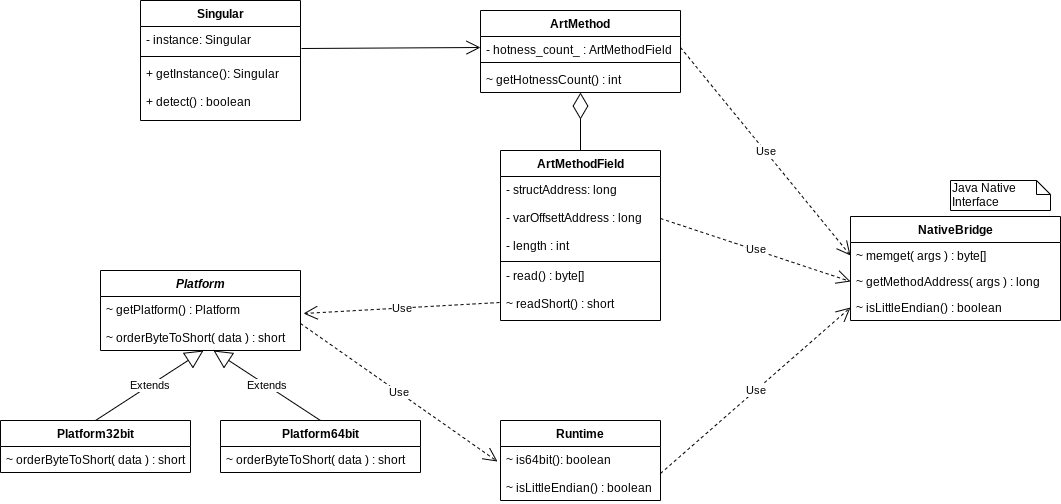
\includegraphics[width=1.2\textwidth]{figures/Singular}
\caption[Diagramma delle classi di Singular]{diagramma delle classi di Singular
\label{fig:singular_uml}}
\end{figure}

\subsection*{Codice nativo}

L'utilizzo del codice nativo C/C++ è necessario per poter leggere dalla memoria primaria l'indirizzo degli \emph{ArtMethod} e l'\emph{hotness\_count} a esso associato.
La classe \emph{Java} che implementa i metodi nativi attraverso la \emph{Java Native Interface} è \emph{NativeBridge}.

\begin{lstlisting}[language = Java , frame = trBL , firstnumber = 1 , escapeinside={(*@}{@*)}]
final class NativeBridge {
    static {
        System.loadLibrary("singularnative");
    }
    static native byte[] memget(long address, int size);
    static native long getMethodAddress(Method method);
    static native boolean isLittleEndian();
}
\end{lstlisting}

La classe è finale ed è raggiungibile solo dallo stesso package per evitare che sia accessibile dall'esterno.
I corrispondenti metodi dichiarati nella classe \emph{NativeBridge} sono disponibili all'interno della libreria \emph{SingularNative}, che viene caricata in riga 3. Le funzioni vengono implementate nel file \emph{singular\_native.cpp} in questo modo:
\begin{itemize}
    \item \emph{isLittleEndian()}
    \begin{lstlisting}[language = C , frame = trBL , firstnumber = 1 , escapeinside={(*@}{@*)}]
jboolean isLittleEndian(JNIEnv * env, jclass clazz) {
    unsigned int num = 0,*p = &num;
    *(unsigned char *)p = 0xff;
    if (num == 0xff)
        return JNI_TRUE;
    return JNI_FALSE;
}
\end{lstlisting}

Verifica se la CPU è \emph{little endian} provando a invertire i byte assegnando il valore \emph{0xff} a un puntatore a un intero.

    \item \emph{getMethodAddress(Method method)}
\begin{lstlisting}[language = C , frame = trBL , firstnumber = 1 , escapeinside={(*@}{@*)}]
jlong getMethodAddress(JNIEnv * env, jclass clazz, jobject method) {
    return (jlong) env->FromReflectedMethod(method);
}
\end{lstlisting}
Viene ritornato l'indirizzo dell'\emph{artMethod} tramite la funzione \emph{FromReflectedMethod} e convertendo il risultato in \emph{jlong}.

    \item \emph{memget(long address ,int size)}
\begin{lstlisting}[language = C , frame = trBL , firstnumber = 1 , escapeinside={(*@}{@*)}]
jbyteArray android_memget(JNIEnv *env, jclass _cls, jlong src, jint length) {
    jbyteArray dest = env->NewByteArray(length);
    if (dest == NULL)
        return NULL;
    unsigned char *destPnt = (unsigned char*)env->GetByteArrayElements(dest,0);
    unsigned char *srcPnt = (unsigned char*)src;
    for(int i = 0; i < length; ++i)
        destPnt[i] = srcPnt[i];
    env->ReleaseByteArrayElements(dest, (jbyte *)destPnt, 0);
    return dest;
}
\end{lstlisting}
Tramite la funzione \emph{NewByteArray} viene allocato un array di lunghezza \emph{length}. Poi viene creato il puntatore alla zona di memoria di destinazione attraverso la funzione \emph{GetByteArrayElements}, e viene copiato l'array sorgente nell'array destinazione.
Tramite la funzione \emph{ReleaseByteArrayElements} viene rilasciata la memoria, e infine ritornato l'array \emph{dest}.
\end{itemize}


\subsection*{Codice java}

Le operazione che esegue \emph{Singular} per leggere il valore dell'\emph{hotness\_count} si possono riassumere in:
\begin{enumerate}
    \item Recupero della classe \emph{ActivityThread} e del metodo \emph{currentActivityThread}:
\begin{lstlisting}[language = C , frame = trBL , firstnumber = 1 , escapeinside={(*@}{@*)}]
Class target = Class.forName("android.app.ActivityThread");
Method curActivityThread = target.getDeclaredMethod("currentActivityThread");
\end{lstlisting}
    \item Creazione di un nuovo oggetto \emph{ArtMethod}, contenente l'indirizzo dell'oggetto \emph{ActivityThread} e l'istanza di un oggetto \emph{ArtMethodField} contenente l'offset e la lunghezza del campo \emph{hotness\_count}:
\begin{lstlisting}[language = C , frame = trBL , firstnumber = 1 , escapeinside={(*@}{@*)}]
ArtMethod(Method associatedMethod) {
    long methodAddress = NativeBridge.getMethodAddress(associatedMethod);
    hotness_count_ = new ArtMethodField(methodAddress, HOTNESS_COUNT_OFFSET, HOTNESS_COUNT_LENGTH);
}
\end{lstlisting}    
    \item Lettura del campo \emph{hotness\_count} grazie al metodo \emph{read} della classe \emph{ArtMethodField}. Prima di eseguire questa operazione viene controllata l'architettura del sistema operativo, tramite la classe \emph{Platform}:
\begin{lstlisting}[language = C , frame = trBL , firstnumber = 1 , escapeinside={(*@}{@*)}]
private byte[] read() {
    return NativeBridge.memget(structAddress + varOffsetAddress,length);
}
\end{lstlisting}       

    \item Viene eseguito il codice nativo della funzione \emph{memget} e viene ritornato il valore legato all'\emph{hotness\_count}, sul quale controllare l'ambiente di esecuzione. Nel caso in cui l'ambiente di esecuzione fosse virtuale, viene segnalato sull'\emph{\gls{activityg}} dell'applicazione \emph{Singular} di supporto.
\end{enumerate}

\newpage


\section{Efficienza}

\emph{Singular} è stata testata su un ampia gamma di dispositivi diversi tra loro, con diverse applicazioni di virtualizzazione. I risultati sono visibili in Tab. \ref{tab:singular_device_tests}.
Nel caso l'applicazione di virtualizzazione non fosse compatibile con la versione di \emph{Android}, il campo della tabella è vuoto.


\begin{table} [H]

\makebox[1 \textwidth][c]{       %centering table
\resizebox{1.2 \textwidth}{!}{   %resize table


\begin{tabular}{l|lllllllllll}    \toprule
\emph{device}  & native & A1 & A2 & A3 & A4 & A5 & A6 & A7 & A8 & DroidPlugin & Màscara\\\midrule
\row Xiaomi mi10 - Android 10 arm64 & false & true & true & true &   & true & true &  &      \\ 
\row Xiaomi mi9 - Android 10 arm64 & false & true & true & true &   & true & true &  &      \\ 
\row Xiaomi mi9t - Android 9 arm64 & false & true & true & true &   & true & true &  & & true & true     \\ 
\row Xiaomi mi9t Pro - Android 10 arm64 & false & true & true & true &   & true & true &  &      \\ 
\row Oneplus 3 - Android 8.1 arm64 & false & true & true & true & true  & true & true & true & true & true & true    \\ 
\row Oneplus 6 - Android 10 arm64 & false & true & true & true &   & true & true &  &     \\ 
\row Oneplus 6t - Android 10 arm64 & false & true & true & true &   & true & true &  &      \\ 
\row Samsung Galaxy S8 - Android 9 arm64& false & true & true & true &   & true & true &  &  & true & true       \\ 
\row Samsung Galaxy A70 - Android 10 arm64 & false & true & true & true &   & true & true &  &     \\ 
\row Samsung Galaxy S4 i9505 - Android 8 (AOSP) armeabi-v7 & false & true & true & true & true  & true & true & true & true & true & true    \\ 
\row LG G4 - Android 8 arm64 & false & true & true & true & true  & true & true & true & true  & true & true    \\  \bottomrule \hline
\end{tabular}



}
}
\caption[Tabella dei test di Singular]{Tabella dei test di Singular \\ false se l’ambiente rilevato è nativo, true se l’ambiente rilevato è virtualizzato \\ A1 = com.lbe.parallel.intl \\ A2 = com.ludashi.dualspace \\ A3 = 
info.cloneapp.mochat.in.goast \\ A4 = 
com.parallel.space.lite \\ A5 =
com.exelliance.multiaccounts \\ A6 =
com.ludashi.superboost \\ A7 =
com.in.parallel.accounts \\ A8 =
com.polestar.domultiple}
\label{tab:singular_device_tests}
\end{table}



\emph{Singular} è stato progettato in modo da mitigare ogni possibilità di \emph{\gls{hookg}} cercando di utilizzare operatori logici al posto di metodi, i quali possono essere intercettati da framework come \emph{Whale}. 



\newpage
\section{Compatibilità}

\emph{Singular} è compatibile da \emph{Android Oreo 8.0} fino all'ultima versione rilasciata ufficialmente \emph{Android 10}. Come si può vedere in Fig. \ref{fig:androidOSdistribution} \emph{Singular} copre il 60.8\% dei dispositivi, percentuale sempre in aumento con il passare del tempo.

\begin{figure} [H]
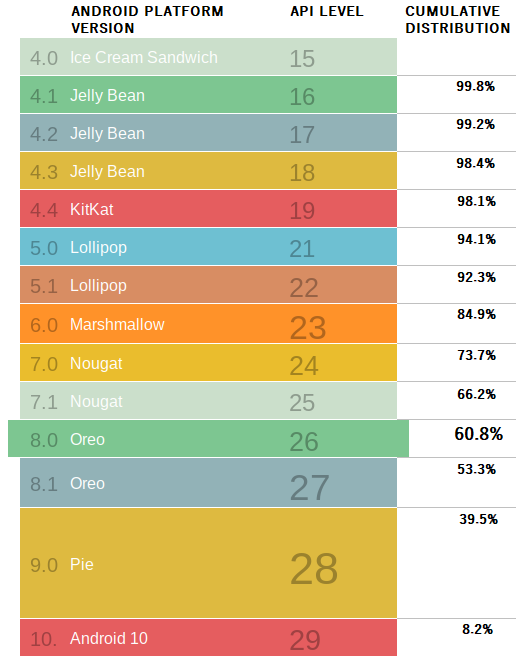
\includegraphics[width=0.8\textwidth]{figures/androidOSdistribution}
\caption[Distrubuzione di Android di Maggio 2020]{Distrubuzione di Android di Maggio 2020
\label{fig:androidOSdistribution}}
\end{figure}

Anche se la percentuale di compatibilità è ancora bassa, la verifica dell'\emph{hotness\_count} per il rilevamento di ambienti virtualizzati risulta essere una tecnica molto più robusta e affidabile rispetto a quelle implementate dalle attuali librerie di identificazione.

\section{Contromisure}

Una possibile contromisura potrebbe essere la riscrittura del valore del field \emph{hotness\_count} ai valori di \emph{Android} nativo. Attraverso il metodo \emph{mprotect} di linux è possibile rimuovere la protezione dalla corrispondente pagina di memoria. 
Le operazioni che dovrebbe eseguire un possibile malware per aggirare questa tecnica di identificazione di ambienti virtualizzati sono:
\begin{itemize}
    \item Implementazione di codice a basso livello per la scrittura in memoria e per la rimozione della protezione;
    \item Riscrittura di tutti gli \emph{hotness\_count} diversi in ambiente virtualizzato: implicherebbe un calo di performance non indifferente per l'applicazione vittima.
\end{itemize}

La fattibilità di una contromisura di questo tipo viene lasciata come test futuro.

\section{Verifica dei requisiti}

I requisiti richiesti iniziali sono stati tutti soddisfatti, come è possibile vedere in Tab. \ref{tab:sodd_requisiti}.


\begin{table} [H]

\begin{tabular}{l|l}    \toprule
\emph{Codice}  & \emph{Esito} \\\midrule
\row RF01 & Soddisfatto \\ 
\row RF02 & Soddisfatto \\ 
\row RF03 & Soddisfatto \\
\row RF04 & Soddisfatto \\
\row RF15 & Soddisfatto \\
\row RV06 & Soddisfatto \\
\row RV17 & Soddisfatto \\
\bottomrule \hline
\end{tabular}


\caption[Tabella del soddisfacimento dei requisiti di Singular]{Tabella del soddisfacimento dei requisiti di Singular}

\label{tab:sodd_requisiti}
\end{table}


%!TEX root = ../dissertation.tex
\chapter{Conclusione}
\label{conclusion}

Gli ambienti virtualizzati in \emph{Android} nascondono molti problemi di sicurezza che attirano molti sviluppatori con scopi sospetti a sfruttarli a loro vantaggio. 
Gli \emph{\gls{hookg}} applicati a \emph{Màscara} per aggirare le librerie di identificazione attualmente esistenti, come \emph{DiPrint} e \emph{Anti-Plugin}, hanno dimostrato la facilità di creazione di un malware che possa inviare dati sensibili a un server esterno, senza che l'utente ne sia a conoscenza.

\emph{Singular}, la libreria creata durante il periodo di stage, è la prima per l'individuazione automatica di ambienti virtualizzati che si basa sulle strutture interne dell'\emph{\gls{artg}} accedendo ai suoi valori direttamente dalla memoria centrale in modo da mitigare la possibilità di applicare degli \emph{\gls{hookg}} cambiando i valori di ritorno delle \emph{API} o funzioni.
In particolare, \emph{Singular} controlla il valore dell'\emph{hotness\_count} al primo avvio di una applicazione, in modo da individuare un ambiente virtualizzato nel caso in cui i metodi della classi \emph{ActivityThread} siano compilati \emph{AoT} e non \emph{JiT}.
Il metodo implementato in \emph{Singular} risulta essere più robusto rispetto alle tecniche utilizzate dalle uniche due librerie attualmente esistenti ma non è negata l'esistenza di possibili contromisure.




\glossarypage


\cleardoublepage
\phantomsection
\addcontentsline{toc}{chapter}{Riferimenti}

\bibliography{mybiblio.bib}


%\printbibliography
% \cleardoublepage
% \phantomsection
%\addcontentsline{toc}{chapter}{Acknowledgments}

% The next two lines define the bibliography style to be used, and
% the bibliography file.
%\bibliographystyle{ACM-Reference-Format}
%\bibliography{mybiblio}


% \clearpage
% \bibliography{references}
% \addcontentsline{toc}{chapter}{References}
% \bibliographystyle{apalike2}

% %!TEX root = ../dissertation.tex
\newpage

% If you do want an image in the colophon:
\begin{figure}
  \vspace{20pt}
  \centering
  \hspace*{-32pt}
  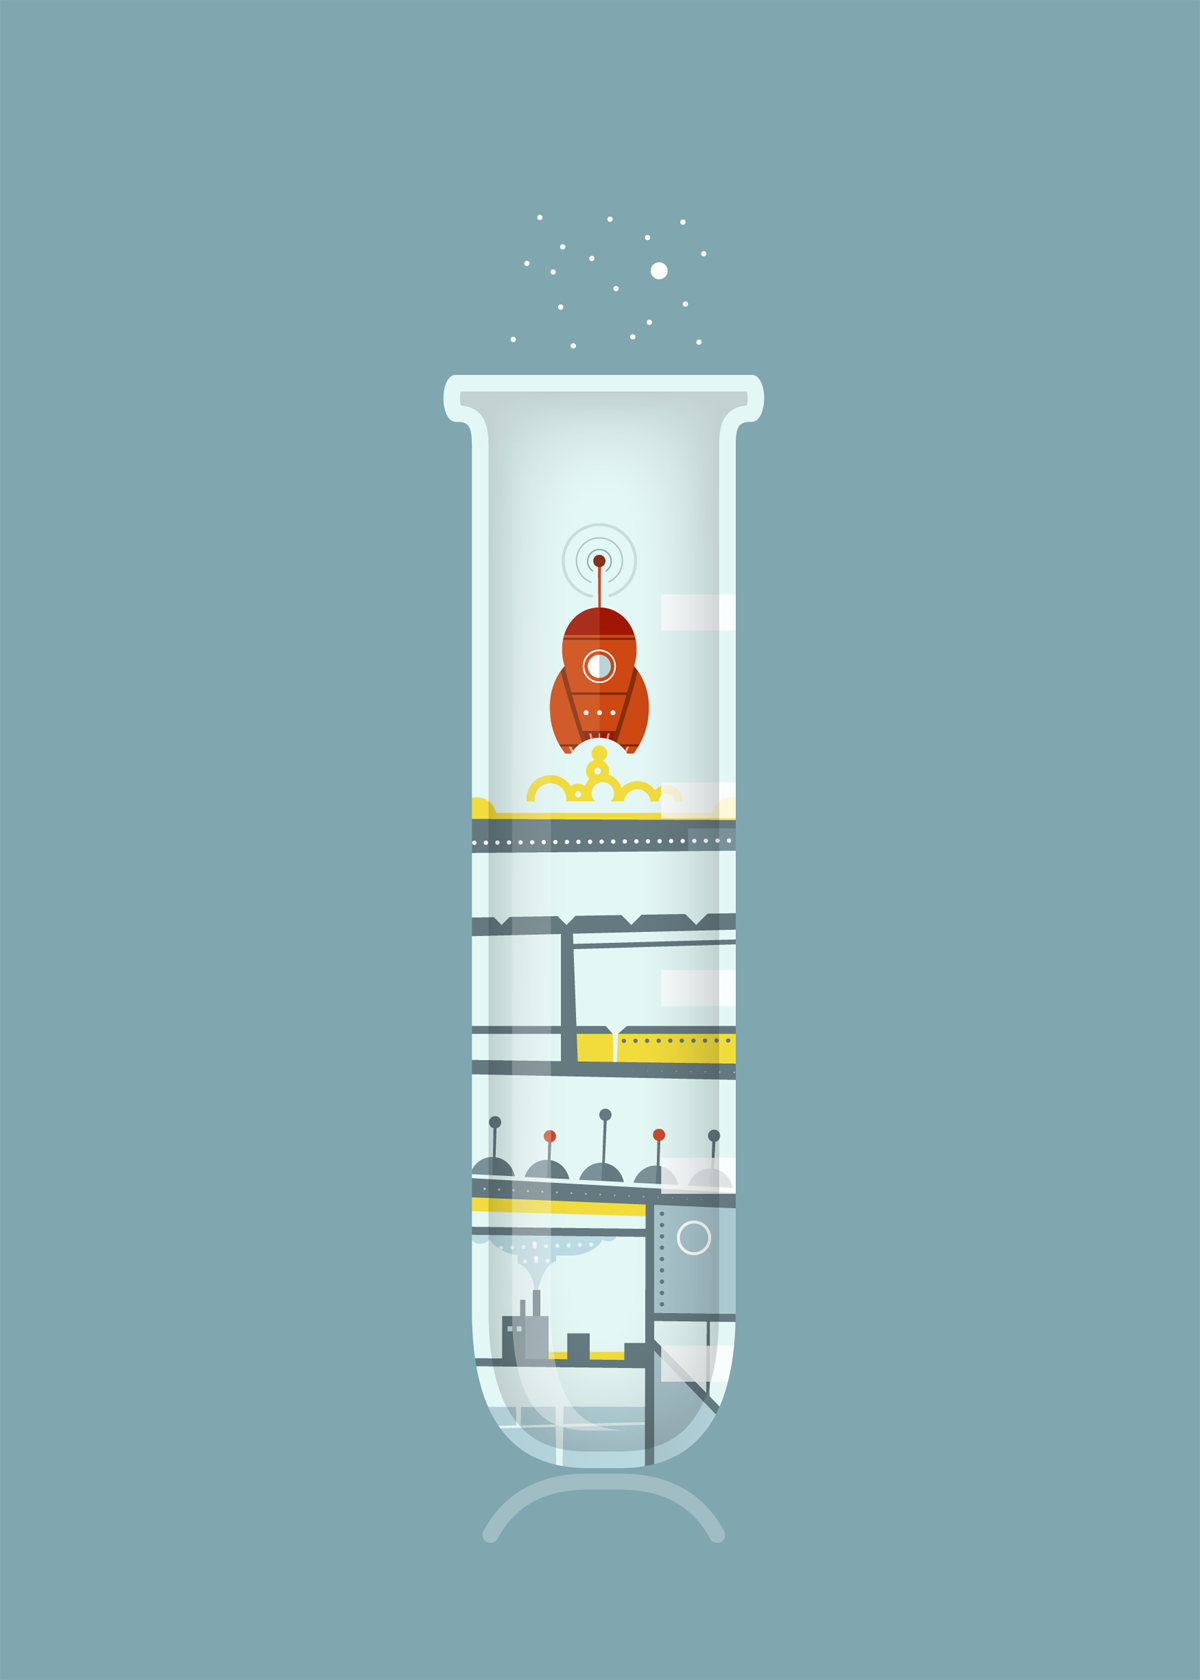
\includegraphics[width=0.42\textwidth]{endmatter/colophon.png}
\end{figure}

% If you don't want an image in the colophon:
% \vspace*{200pt}

\begin{center}
\parbox{200pt}{\lettrine[lines=3,slope=-2pt,nindent=-4pt]{\textcolor{SchoolColor}{T}}{his thesis was typeset} using \LaTeX, originally developed by Leslie Lamport and based on Donald Knuth's \TeX. The body text is set in 11 point Egenolff-Berner Garamond, a revival of Claude Garamont's humanist typeface. The above illustration, \textit{Science Experiment 02}, was created by Ben Schlitter and released under \href{http://creativecommons.org/licenses/by-nc-nd/3.0/}{\textsc{cc by-nc-nd 3.0}}. A template that can be used to format a PhD dissertation with this look \textit{\&} feel has been released under the permissive \textsc{agpl} license, and can be found online at \href{https://github.com/suchow/Dissertate}{github.com/suchow/Dissertate} or from its lead author, Jordan Suchow, at \href{mailto:suchow@post.harvard.edu}{suchow@post.harvard.edu}.}
\end{center}





\end{document}
